\documentclass[a4paper,ngerman,naustrian,DIV=12,BCOR=1cm]{scrbook}
\usepackage[T1]{fontenc}
\usepackage[utf8]{inputenc}
\usepackage{fancyhdr}
\pagestyle{fancy}
\setcounter{secnumdepth}{3}
\usepackage{babel}
\usepackage{textcomp}
\usepackage{url}
\usepackage{makeidx}
\usepackage{float}
\usepackage{wrapfig}
\makeindex
\usepackage{graphicx}
\usepackage{epstopdf}
\PassOptionsToPackage{normalem}{ulem}
\usepackage{ulem}
\usepackage{needspace}
\usepackage[unicode=true,
 bookmarks=true,bookmarksnumbered=false,bookmarksopen=false,
 breaklinks=true,pdfborder={0 0 0},backref=false,colorlinks=false]
 {hyperref}
\hypersetup{pdftitle={sblit},
 pdfauthor={Martin Exner, Andreas Novak, Nikola Szucsich},
 pdfsubject={Diplomarbeit},
 pdfkeywords={Diplomarbeit}}

\makeatletter

%%%%%%%%%%%%%%%%%%%%%%%%%%%%%% LyX specific LaTeX commands.
\pdfpageheight\paperheight
\pdfpagewidth\paperwidth

\voffset10mm

%% Because html converters don't know tabularnewline
\providecommand{\tabularnewline}{\\}

%%%%%%%%%%%%%%%%%%%%%%%%%%%%%% Textclass specific LaTeX commands.
\newcommand{\strong}[1]{\textbf{#1}}
\newcommand{\code}[1]{\texttt{#1}}

%%%%%%%%%%%%%%%%%%%%%%%%%%%%%% User specified LaTeX commands.
%%%%%%%%%%%%
% Latex-Vorspann
\usepackage{lastpage}
\usepackage{listings}
\usepackage{blindtext}

%% geht nicht mit jeder Latex Variante, gibt aber ein schöneres Layout
\usepackage{microtype}

%% Aufzählungen nicht so weit einrücken
\usepackage{enumitem}
%\setitemize{leftmargin=*}

% Serifenschrift für Überschriften
\addtokomafont{disposition}{\rmfamily}

% Serifenschrift für Description-Lists
\setlist[description]{font=\rmfamily}

%\usepackage{caladea}
%\usepackage[T1]{fontenc}
\usepackage{lmodern}

%% für pandoc
%% maximale Breite der Bilder
\setkeys{Gin}{width=0.90\linewidth,keepaspectratio}

\makeatother

\usepackage{listings}
\addto\captionsnaustrian{\renewcommand{\lstlistingname}{Listing}}
\addto\captionsngerman{\renewcommand{\lstlistingname}{Listing}}
\renewcommand{\lstlistingname}{Listing}

% to insert a space after use of an argument-less command depending on what follows (\xspace)
\usepackage{xspace}

% to use with java syntax highlighting
\usepackage{color}

% to draw packet structures
\usepackage{bytefield}

% to include pages from PDF files
\usepackage{pdfpages}

% to place tables exactly here
\usepackage{float}
\restylefloat{table}

% global definitions

\newcommand{\kap}[1]{(\textbf{deprecated}) \link{#1}} % TODO remove

\newcommand{\labellinkt}[1]{\ref{#1} \nameref{#1}}
\newcommand{\labellink}[1]{\hyperref[#1]{\labellinkt{#1}}}
\newcommand{\pagelinkt}[1]{Seite~\pageref{#1}}
\newcommand{\pagelink}[1]{\hyperref[#1]{\pagelinkt{#1}}}
\newcommand{\linkt}[1]{\labellinkt{#1}, \pagelinkt{#1}}
\newcommand{\link}[1]{\hyperref[#1]{\linkt{#1}}}
\newcommand{\siehet}[1]{siehe~\linkt{#1}}
\newcommand{\siehe}[1]{\hyperref[#1]{\siehet{#1}}}
\newcommand{\referenz}[1]{\hyperref[#1]{(\siehet{#1})}}
\newcommand{\abbildung}[1]{(siehe Abbildung \linkt{#1fig})}
\newcommand{\figurelinkt}[1]{Abbildung~\ref{#1}, \nameref{#1}}
\newcommand{\figurelink}[1]{\hyperref[#1]{\figurelinkt{#1}}}
\newcommand{\figurelinkpt}[1]{Abbildung~\ref{#1}, \nameref{#1}, \pagelinkt{#1}}
\newcommand{\figurelinkp}[1]{\hyperref[#1]{\figurelinkpt{#1}}}

\newcommand{\codeline}[1]{\sloppy{\mbox{\code{#1}}}}

\newcommand{\tags}[2]{\hspace{0in}#2}

\newcommand{\sblit}{sblit\xspace}
\newcommand{\sblitg}{\sblit}

\newcommand{\addrkeybits}{2048\xspace}
\newcommand{\addrkeybytes}{256\xspace}

\newcommand{\javaarg}{Argument\xspace}
\newcommand{\javainstvar}{Instanzvariable\xspace}

\newcommand{\cnettype}{org.dclayer.circle}
\newcommand{\cnetattr}{sha1/20}
\newcommand{\cnetid}{\cnettype{} \cnetattr{}}

\newcommand{\msg}[1]{#1 Message}
\newcommand{\msgpl}[1]{#1 Messages}

\newcommand{\comp}[1]{#1 Component}

\newcommand{\isprotomsgtype}{Message Type}
\newcommand{\isprotomsgdata}{Message Data}

\newcommand{\flexnumfield}{\glslink{fnumc}{FlexNum, 1 -- 9 Bytes}}
\newcommand{\netpktfield}{\glslink{netpkt}{NetworkPacket, $N$ Bytes}}

\newcommand{\descriptionitem}[1]{\item[{#1}] \hfill \nopagebreak \\}
\newcommand{\datei}[1]{\textit{#1}}

\newcommand{\const}[1]{\code{#1}}

% shamelessly stolen from http://tex.stackexchange.com/a/35943 and modified
\newcommand{\namesigdate}[2][8cm]{
    \begin{tabular}{@{}p{#1}@{}}
        \\
        \\
        \\
        \\
        \hrule \\
        \small{#2}
    \end{tabular}
}


\newcommand{\keycrsat}{RSA Key}

\newcommand{\keycrsa}{\hyperref[dcl-keyc-rsa]{\keycrsat}}

\newcommand{\keycbytefield}{}

\newcommand{\keycrsabytefield}{}


\newcommand{\bmcpconnectreqt}{Connect Request}
\newcommand{\bmcpconnectrept}{Connect Reply}
\newcommand{\bmcpopenchreqt}{Open Channel Request}
\newcommand{\bmcpchblockstatreqt}{Channel Block Status Request}
\newcommand{\bmcpchblockstatrept}{Channel Block Status Report}
\newcommand{\bmcpkillt}{Kill}
\newcommand{\bmcpthrottlet}{Throttle}
\newcommand{\bmcpdisconnectt}{Disconnect}
\newcommand{\bmcpackt}{Ack}
\newcommand{\bmcpchprotoreqt}{Change Protocol Request}
\newcommand{\bmcpcryptoinitt}{Crypto Init}

\newcommand{\bmcpconnectreq}{\hyperref[dcl-bmcp-connectreq]{\bmcpconnectreqt}}
\newcommand{\bmcpconnectrep}{\hyperref[dcl-bmcp-connectrep]{\bmcpconnectrept}}
\newcommand{\bmcpopenchreq}{\hyperref[dcl-bmcp-openchreq]{\bmcpopenchreqt}}
\newcommand{\bmcpchblockstatreq}{\hyperref[dcl-bmcp-chblockstatreq]{\bmcpchblockstatreqt}}
\newcommand{\bmcpchblockstatrep}{\hyperref[dcl-bmcp-chblockstatrep]{\bmcpchblockstatrept}}
\newcommand{\bmcpkill}{\hyperref[dcl-bmcp-kill]{\bmcpkillt}}
\newcommand{\bmcpthrottle}{\hyperref[dcl-bmcp-throttle]{\bmcpthrottlet}}
\newcommand{\bmcpdisconnect}{\hyperref[dcl-bmcp-disconnect]{\bmcpdisconnectt}}
\newcommand{\bmcpack}{\hyperref[dcl-bmcp-ack]{\bmcpackt}}
\newcommand{\bmcpchprotoreq}{\hyperref[dcl-bmcp-chprotoreq]{\bmcpchprotoreqt}}
\newcommand{\bmcpcryptoinit}{\hyperref[dcl-bmcp-cryptoinit]{\bmcpcryptoinitt}}

\newcommand{\bmcpbytefield}{}

\newcommand{\bmcpconnectreqbytefield}{}
\newcommand{\bmcpconnectrepbytefield}{}
\newcommand{\bmcpopenchreqbytefield}{}
\newcommand{\bmcpchblockstatreqbytefield}{}
\newcommand{\bmcpchblockstatrepbytefield}{}
\newcommand{\bmcpkillbytefield}{}
\newcommand{\bmcpthrottlebytefield}{}
\newcommand{\bmcpdisconnectbytefield}{}
\newcommand{\bmcpackbytefield}{}
\newcommand{\bmcpchprotoreqbytefield}{}
\newcommand{\bmcpcryptoinitbytefield}{}


\newcommand{\crispneighreqt}{Neighbor Request}

\newcommand{\crispneighreq}{\hyperref[dcl-crisp-neighreq]{\crispneighreqt}}

\newcommand{\crispbytefield}{}

\newcommand{\crispneighreqbytefield}{}


\newcommand{\isprotocbnt}{Connection Base Notice}
\newcommand{\isprotonjnt}{Network Join Notice}
\newcommand{\isprotoireqt}{Integration Request}
\newcommand{\isprotoicreqt}{Integration Connect Request}
\newcommand{\isprotoccrept}{Crypto Challenge Reply}
\newcommand{\isprotoccreqt}{Crypto Challenge Request}
\newcommand{\isprotollarept}{LLA Reply}
\newcommand{\isprotollareqt}{LLA Request}
\newcommand{\isprotonlnt}{Network Leave Notice}
\newcommand{\isprotoacdt}{Application Channel Data}
\newcommand{\isprototst}{Trusted Switch}
\newcommand{\isprotoversiont}{Version}
\newcommand{\isprotonpt}{Network Packet}
\newcommand{\isprotoacsat}{Application Channel Slot Assign}

\newcommand{\isprotocbn}{\hyperref[dcl-isproto-cbn]{\isprotocbnt}}
\newcommand{\isprotonjn}{\hyperref[dcl-isproto-njn]{\isprotonjnt}}
\newcommand{\isprotoireq}{\hyperref[dcl-isproto-ireq]{\isprotoireqt}}
\newcommand{\isprotoicreq}{\hyperref[dcl-isproto-icreq]{\isprotoicreqt}}
\newcommand{\isprotoccrep}{\hyperref[dcl-isproto-ccrep]{\isprotoccrept}}
\newcommand{\isprotoccreq}{\hyperref[dcl-isproto-ccreq]{\isprotoccreqt}}
\newcommand{\isprotollarep}{\hyperref[dcl-isproto-llarep]{\isprotollarept}}
\newcommand{\isprotollareq}{\hyperref[dcl-isproto-llareq]{\isprotollareqt}}
\newcommand{\isprotonln}{\hyperref[dcl-isproto-nln]{\isprotonlnt}}
\newcommand{\isprotoacd}{\hyperref[dcl-isproto-acd]{\isprotoacdt}}
\newcommand{\isprotots}{\hyperref[dcl-isproto-ts]{\isprototst}}
\newcommand{\isprotoversion}{\hyperref[dcl-isproto-version]{\isprotoversiont}}
\newcommand{\isprotonp}{\hyperref[dcl-isproto-np]{\isprotonpt}}
\newcommand{\isprotoacsa}{\hyperref[dcl-isproto-acsa]{\isprotoacsat}}

\newcommand{\isprotobytefield}{}

\newcommand{\isprotocbnbytefield}{}
\newcommand{\isprotonjnbytefield}{}
\newcommand{\isprotoireqbytefield}{}
\newcommand{\isprotoicreqbytefield}{}
\newcommand{\isprotoccrepbytefield}{}
\newcommand{\isprotoccreqbytefield}{}
\newcommand{\isprotollarepbytefield}{}
\newcommand{\isprotollareqbytefield}{}
\newcommand{\isprotonlnbytefield}{}
\newcommand{\isprotoacdbytefield}{}
\newcommand{\isprototsbytefield}{}
\newcommand{\isprotoversionbytefield}{}
\newcommand{\isprotonpbytefield}{}
\newcommand{\isprotoacsabytefield}{}


\newcommand{\asprotocryptoresponset}{Key Crypto Response}
\newcommand{\asprotokeynumt}{Key Number Response}
\newcommand{\asprotojoindefnetst}{Join Default Networks}
\newcommand{\asprotoappchacceptt}{Application Channel Accept}
\newcommand{\asprotoslotassignt}{Slot Assign}
\newcommand{\asprotokeyenct}{Key Encrypt}
\newcommand{\asprotoappchinreqt}{Application Channel Incoming Request}
\newcommand{\asprotoappchdatat}{Application Channel Data}
\newcommand{\asprotoappchconnectedt}{Application Channel Connected}
\newcommand{\asprotokeyencblocksizereqt}{Key Encryption Block Size Request}
\newcommand{\asprotokeydect}{Key Decrypt}
\newcommand{\asprotoaddrpubkeyt}{Address Public Key}
\newcommand{\asprotoappchoutreqt}{Application Channel Outgoing Request}
\newcommand{\asprotodatat}{Data}
\newcommand{\asprotogenkeyt}{Generate Key}
\newcommand{\asprotojoinnett}{Join Network}
\newcommand{\asprotorevisiont}{Revision}

\newcommand{\asprotocryptoresponse}{\hyperref[dcl-asproto-cryptoresponse]{\asprotocryptoresponset}}
\newcommand{\asprotokeynum}{\hyperref[dcl-asproto-keynum]{\asprotokeynumt}}
\newcommand{\asprotojoindefnets}{\hyperref[dcl-asproto-joindefnets]{\asprotojoindefnetst}}
\newcommand{\asprotoappchaccept}{\hyperref[dcl-asproto-appchaccept]{\asprotoappchacceptt}}
\newcommand{\asprotoslotassign}{\hyperref[dcl-asproto-slotassign]{\asprotoslotassignt}}
\newcommand{\asprotokeyenc}{\hyperref[dcl-asproto-keyenc]{\asprotokeyenct}}
\newcommand{\asprotoappchinreq}{\hyperref[dcl-asproto-appchinreq]{\asprotoappchinreqt}}
\newcommand{\asprotoappchdata}{\hyperref[dcl-asproto-appchdata]{\asprotoappchdatat}}
\newcommand{\asprotoappchconnected}{\hyperref[dcl-asproto-appchconnected]{\asprotoappchconnectedt}}
\newcommand{\asprotokeyencblocksizereq}{\hyperref[dcl-asproto-keyencblocksizereq]{\asprotokeyencblocksizereqt}}
\newcommand{\asprotokeydec}{\hyperref[dcl-asproto-keydec]{\asprotokeydect}}
\newcommand{\asprotoaddrpubkey}{\hyperref[dcl-asproto-addrpubkey]{\asprotoaddrpubkeyt}}
\newcommand{\asprotoappchoutreq}{\hyperref[dcl-asproto-appchoutreq]{\asprotoappchoutreqt}}
\newcommand{\asprotodata}{\hyperref[dcl-asproto-data]{\asprotodatat}}
\newcommand{\asprotogenkey}{\hyperref[dcl-asproto-genkey]{\asprotogenkeyt}}
\newcommand{\asprotojoinnet}{\hyperref[dcl-asproto-joinnet]{\asprotojoinnett}}
\newcommand{\asprotorevision}{\hyperref[dcl-asproto-revision]{\asprotorevisiont}}

\newcommand{\asprotobytefield}{}

\newcommand{\asprotocryptoresponsebytefield}{}
\newcommand{\asprotokeynumbytefield}{}
\newcommand{\asprotojoindefnetsbytefield}{}
\newcommand{\asprotoappchacceptbytefield}{}
\newcommand{\asprotoslotassignbytefield}{}
\newcommand{\asprotokeyencbytefield}{}
\newcommand{\asprotoappchinreqbytefield}{}
\newcommand{\asprotoappchdatabytefield}{}
\newcommand{\asprotoappchconnectedbytefield}{}
\newcommand{\asprotokeyencblocksizereqbytefield}{}
\newcommand{\asprotokeydecbytefield}{}
\newcommand{\asprotoaddrpubkeybytefield}{}
\newcommand{\asprotoappchoutreqbytefield}{}
\newcommand{\asprotodatabytefield}{}
\newcommand{\asprotogenkeybytefield}{}
\newcommand{\asprotojoinnetbytefield}{}
\newcommand{\asprotorevisionbytefield}{}



% listings

\definecolor{javastring}{rgb}{0.6,0,0} % for strings
\definecolor{javacomment}{rgb}{0.25,0.5,0.35} % comments
\definecolor{javakeyword}{rgb}{0.5,0,0.35} % keywords
\definecolor{javadoc}{rgb}{0.25,0.35,0.75} % javadoc

\newcommand{\javalisting}{\lstset{language=Java, breaklines=true, basicstyle=\ttfamily, keywordstyle=\color{javakeyword}\bfseries, stringstyle=\color{javastring}, commentstyle=\color{javacomment}, morecomment=[s][\color{javadoc}]{/**}{*/}, numbers=left, numberstyle=\tiny, stepnumber=1, numbersep=5pt, tabsize=4, showspaces=false, showstringspaces=false, frame=single}}

\newcommand{\messagestart}{\begin{figure}[p] \centering \begin{bytefield}[bitwidth=2em]{8}}
\newcommand{\messageend}[1]{\end{bytefield} \par \protect\caption{\gls{#1}} \label{#1fig} \end{figure}}


\newcommand{\listingstart}[1]{\javalisting \begin{lstlisting}[caption={#1},captionpos=b]}

%\lstset{numbers=right, numberstyle=\tiny, stepnumber=2, numbersep=5pt, showspaces=false, frame=single}


% glossaries
\usepackage[toc,acronym]{glossaries}
\makeglossaries

% DO NOT ADD ENTRIES HERE
% Add them in your *_glossary.tex file instead

\newglossaryentry{partnership}{
	name=Partnerschaft,
	plural=Partnerschaften,
	description={Um Dateien/Dateiblöcke extern speichern zu können, muss eine
	sogenannte Partnerschaft mit anderen Geräten eingangen werden, bei der man
	Dateiblöcke auf den jeweilig anderen Geräten speichert, während man selber
	Speicherplatz für diese Partner freigibt, in dem deren verschlüsselte
	Dateiblöcke	gespeichert werden}
}

\newglossaryentry{syncpartner}{
	name=Synchronisationspartner,
	plural=Synchronisationspartner,
	description={Gerät mit dem der \sblit-Ordner synchronisiert wird}
}

\newglossaryentry{p2plink}{
	name=Peer-to-Peer-Link,
	plural=Peer-to-Peer-Links,
	description={Ein direkte Verbindung zwischen zwei Endgeräten}
}

\newglossaryentry{syncconflict}{
	name=Synchronisationskonflikt,
	plural=Synchronisationskonflikte,
	description={Wenn eine synchronisierte Datei von zwei Rechnern bearbeitet wird,
	ohne, dass sie in der Zwischenzeit synchronisert werden konnte. Es existieren
	dann zwei Versionen der gleichen Datei. Man spricht dann von einem Konflikt}
}

\newglossaryentry{filecloud}{
	name=Filecloud,
	description={Externer Speicher im Internet, auf dem Dateien gespeichert werden
	können. Meistens bestehend aus einem oder mehreren Servern}
}


\newglossaryentry{cl}{
	name=Kommunikationsschicht,
	description={Eine Schicht im netzwerktechnischen Sinne, die zur Kommunikation verwendet wird},
	see={[Siehe:]{gls_dcl}}
}

\newglossaryentry{p2pnet}{
	name=Peer-to-Peer-Netzwerk,
	description={Ein Kommunikationsnetzwerk, in dem die einzelnen Kommunikationspartner im Gegensatz zu einer klassischen Client-Server-Infrastruktur direkt miteinander kommunizieren}
}

\newglossaryentry{gls_dcl}{
	name=Decentralized Communication Layer,
	description={Die auf einem dezentralen \gls{p2pnet} basierende \gls{cl}, die \sblit zur Kommunikation benutzt}
}

\newacronym[see={[Glossar:]{gls_dcl}}]{dcl}{DCL}{Decentralized Communication Layer\glsadd{gls_dcl}}

\newglossaryentry{aenc}{
	name=Asymmetrisches Verschlüsselungsverfahren,
	description={Verschlüsselungsverfahren, bei dem zur Entschlüsselung einer Nachricht ein anderer Schlüssel verwendet wird, als zur Verschlüsselung verwendet wurde},
	see={[Siehe:]{rsa}}
}

\newglossaryentry{rsa}{
	name=RSA,
	description={\gls{aenc}, benannt nach und erstmals veröffentlich von Ron Rivest, Adi Shamir and Leonard Adleman \cite{wikipedia:rsa}},
	see={[Siehe:]{aenc}}
}

\newglossaryentry{hash}{
	name=Hashalgorithmus,
	plural=Hashalgorithmen,
	description={Algorithmus, der eine große Eingabemenge auf eine kleinere Zielmenge (\gls{hashval}) abbildet \cite{wikipedia:hash}}
}

\newglossaryentry{Hash}{
	name=Hash,
	description={Im Quellcode von \gls{dcl} definierte Klasse zur Anwendung von \glspl{hash} auf \gls{Data}-Objekte}
}

\newglossaryentry{hashval}{
	name=Hashwert,
	plural=Hashwerte,
	description={Ergebnis bei Anwendung eines \gls{hash}}
}

\newglossaryentry{digestlength}{
	name=Digest Length,
	description={Die Länge der \glspl{hashval} eines \gls{hash}}
}

\newglossaryentry{cnt}{
	name=CircleNetworkType,
	description={Standard \gls{nt} im \gls{dcl}},
	see={[Siehe:]{nt}}
}

\newglossaryentry{nt}{
	name=Network Type,
	description={Beschreibt ein Netzwerk innerhalb des \gls{dcl} samt Adresskonzept und Routingverfahren},
	see={[Siehe:]{cnt}}
}

\newglossaryentry{Data}{
	name=Data,
	description={Im Quellcode von \gls{dcl} definierte Klasse zur Speicherung von Binärdaten}
}

\newglossaryentry{partnerdevice}{
	name=Partnergerät,
	description={Ein Gerät eines anderen \sblit-Nutzers, mit dem eine Partnerschaft besteht}
}
\newglossaryentry{authreq}{
	name=Authenticity Request,
	description={Eine Nachricht zur Anforderung einer Challenge, um die Authentizität des Gegenübers sicherzustellen}
}
\newglossaryentry{authres}{
	name=Authenticity Response,
	description={Die Antwort auf den \gls{authreq}, um die eigene Authentizität zu beweisen}
}
\newglossaryentry{filereq}{
	name=File Request,
	description={Die Anfrage an das Gegenüber, ob eine Datei benötigt wird}
}
\newglossaryentry{fileres}{
	name=File Response,
	description={Die Antwort auf einen File Request, der eine Datei akzeptiert oder verweigert}
}
\newglossaryentry{filemsg}{
	name=File Message,
	description={Die eigentliche Übertragung einer Datei}
}
\newglossaryentry{filedel}{
	name=File Delete Message,
	description={Eine Nachricht, die dazu dient, Geräte über eine Löschung einer Datei zu informieren}
}
\newglossaryentry{logfile}{
	name=Logfile,
	description={Die Datei, in der der Versionsverlauf einer Datei steht. Außerdem werden hier die Geräte, auf denen die Datei schon vorhanden ist, gelistet}
}
\newglossaryentry{refdev}{
	name=Device Refresh Message,
	description={Eine Nachricht, die eine aktualisierte Version von Partnergeräten oder eigenen Geräten enthält}
}
\newglossaryentry{partfilereq}{
	name=Partner File Request,
	description={Ein \gls{filereq} an ein Partnergerät \referenz{Partnergerät} oder von einem Partnergerät}
}
\newglossaryentry{partfileres}{
	name=Partner File Response,
	description={Ein \gls{fileres} an ein Partnergerät \referenz{Partnergerät} oder von einem Partnergerät}
}
\newglossaryentry{partfilemsg}{
	name=Partner File Message,
	description={Eine \gls{filemsg} an ein Partnergerät \referenz{Partnergerät} oder von einem Partnergerät}
}
\newglossaryentry{partfiledel}{
	name=Partner File Delete Message,
	description={Eine \gls{filedel} an ein Partnergerät \referenz{Partnergerät} oder von einem Partnergerät}
}
\newglossaryentry{watchservice}{
	name=\code{WatchService},
	description={Eine Schnittstelle zum Filesystem, welche benachrichtigt wird, wenn sich eine Datei in einem bestimmten Ordner ändert}
}
\newglossaryentry{watchkey}{
	name=\code{WatchKey},
	description={Ein Objekt, das vom \gls{watchservice} erstellt wird, wenn sich etwas in dem zu überwachenden Ordner ändert}
}
%\newacronym[see={[Glossar:]{authreq}}]{authreq}{AuthReq}{Authenticity Request\glsadd{authreq}}



\newglossaryentry{gls_gui}{
	name=Graphical User Interface,
	description={Eine grafische Oberfläche für Benutzer, um eine Anwendung komfortabel bedienen zu können}
}

\newglossaryentry{versionconflict}{
	name=Versionskonflikt,
	plural=Versionskonflikte,
	description={Wenn eine synchronisierte Datei auf zwei Rechnern gleichzeitig
	bearbeitet wird, tritt ein Konflikt auf, da zwei Versionen der gleichen Datei
	existieren und somit keine der Versionen synchronisiert und von allen
	übernommen werden kann.}
}

\newacronym[see={[Glossar:]{gls_gui}}]{gui}{GUI}{Graphical User Interface\glsadd{gls_gui}}

\newglossaryentry{Prix Ars Electronica}{
	name=Prix Ars Electronica,
	description={Ist der traditionsreichste Medienkunstwettbewerb wird gemeinsam
  von der Ars Electronica Linz GmbH und dem ORF Oberösterreich in Zusammenarbeit mit dem OK Offenes
  Kulturhaus Oberösterreich und dem Brucknerhaus Linz veranstaltet.
}
}



\bytefieldsetup{
  rightcurlyspace=0pt,
  leftcurlyspace=12pt
}

\begin{document}
%%%%%%
% Weitere Einstellungen siehe Latex-Vorspann%%%%%%%%%%%%%%%%%%%%%%%%%%%%%%%%%%%%%%%%%%%%%%%%%%%%%%%%%%%%%%%%%%%%%%%%%%%%%%%%%%
% falls man die erste Zeile der Absätze nicht einrücken will
% dann sollte man aber etwas mehr Abstand zwischen den Absätzen erlauben
%%\setlength{\parindent}{0pt}
%%\setlength{\parskip}{1.5ex plus0.5ex minus0.5ex}
% Auch Fußnoten bündig ausrichten
\deffootnote[]{1em}{1em}{\textsuperscript{\thefootnotemark\ }}
% Listen etwas wenige einrücken, erfordert enumitem
\setitemize{leftmargin=*}

%%%%%%%%%%%%%%%%%%%%%%%%%%%%%%%%%%%%%%%%%%%%%%%%%%%%%%%%%%%%%%%%%%%%%%%%%%%%%%%%%%
%  Kopf und Fußzeilen -- links und rechts verschieden
\newcommand{\kopfseitenummer}{{\bfseries \thepage}}
\newcommand{\kopfkapl}{{\bfseries\leftmark}}
\newcommand{\kopfkapr}{{\bfseries\rightmark}}
\newcommand{\kopfbild}{}%\includegraphics[width=25mm]{HTL3RLogoRGB}}
\newcommand{\kopfHTL}{Höhere Technische Bundeslehranstalt Wien 3, \\Rennweg 	Abteilung für Informationstechnologie}
\renewcommand{\chaptermark}[1]%
  {\thispagestyle{fancy}\markboth{\thechapter.\ #1}{}}%\thispagestyle{fancy}
\renewcommand{\headrulewidth}{0.2pt}
%\lhead[\fancyplain{\kopfbild}{\kopfbild}]% li aussen
%      {\fancyplain{\kopfHTL}{\kopfHTL}}% re innen
%\rhead[\kopfHTL]% li innen
%      {\kopfbild}% re aussen

%% mit kapitelautor kann man den Autor festlegen oder auf leer setzen - steht dann in der Fußzeile.
\newcommand{\kapitelautor}{}

%%%
% Alternative: am Rand (Marginale)
%\setlength{\marginparsep}{-5mm}
%\mbox{}\marginpar{\raggedleft\hspace{0pt}Autor: Hans Huber}

%% kopf links: [linke] und {rechte} Seite

\lhead[\kopfbild]{\fancyplain{}{\kopfkapl}}
\rhead[\fancyplain{}{\kopfkapr}]{\kopfbild}
\chead{}

\lfoot[\kopfseitenummer]{\kapitelautor}
\cfoot[]{}
\rfoot[\kapitelautor]{\kopfseitenummer}

%%%%%Anfang Titelseite
\pagenumbering{roman}
\title{Diplomarbeit}
\begin{titlepage}
\begin{minipage}[b]{1\columnwidth}
\parbox[b]{50mm}{\includegraphics[width=45mm]{HTL3RLogoRGB}}
\hfill
\parbox[b]{130mm}{\footnotesize \textsc{Höhere Technische Bundeslehranstalt} Wien 3, Rennweg\\
IT \& Mechatronik\\
\\
HTL Rennweg :: Rennweg 89b\\
A-1030 Wien :: Tel +43 1 24215-10 :: Fax DW 18
}\\
\mbox{}
\end{minipage}

\vspace{1cm}


\begin{center}
\textbf{\LARGE{}Diplomarbeit}{\large{}}\\
{\large{}\vspace{15mm}
 }\textbf{\large{}sblit}\\
 \vspace{15mm}
 ausgeführt an der\\
 Höheren Abteilung für Informationstechnologie/Netzwerktechnik\\
 der Höheren Technischen Lehranstalt Wien 3 Rennweg\\
 \vspace{1cm}
 im Schuljahr 2014/2015\\
 \vspace{1cm}
 durch\\
 \vspace{0.5cm}
\textbf{\large{}Martin Exner}\\
\textbf{\large{}Andreas Novak}\\
\textbf{\large{}Nikola Szucsich}\\

\par\end{center}{\large \par}

\begin{center}
\vspace{20mm}
 \normalsize unter der Anleitung von\\
 \vspace{0.5cm}
 August Hörandl
\par\end{center}

\begin{center}
\vspace{5mm}
Wien, \today
\par\end{center}

\end{titlepage}%%%%%%%%%%%%%%%%%%%%% Ende Titelseite %%%%%%%%%%%%%%%%%%%%%%


\chapter*{Kurzfassung}

% Auf Seiten mit einem neuen Kapitel ist keine Kopfzeile -- kann man sich aber wünschen
\markboth{Kurzfassung}{}
\thispagestyle{fancy}

Diese Diplomarbeit zielt darauf ab, einen Dienst zur Synchronisation von Dateien
über das Internet in der Form freier Software zu schaffen.
Zentrale Stellen wie Server sollen dabei im Sinne der Sicherheit vor Eingriffen
durch Unbefugte nicht eingesetzt werden.
Statt der Zwischenspeicherung von Daten auf Cloudspeicher eines herkömmlichen
Anbieters werden Daten in verschlüsselten Blöcken auf den Geräten anderer Nutzer
zwischengespeichert.

An die Stelle einer klassischen Client-Server-Infrastruktur tritt ein
dezentrales Peer-to-Peer-Netzwerk.
Dadurch und durch die Verteilung von Daten auf Geräte anderer Teilnehmer
auftretende Problemstellungen sollen im Rahmen dieser Diplomarbeit gelöst
werden.
Dazu zählen dezentrale Adressierung, dezentrales Routing, Fairness von
gegenseitiger Speicherfreigabe, Sicherheit und Effizienz von Kommunikation und
Synchronisation sowie Behandlung von Synchronisationskonflikten.



\chapter*{Abstract}

% mit Kopfzeile
\markboth{Abstract}{}
\thispagestyle{fancy}

That's why.

\blindtext[1]



\chapter*{Ehrenwörtliche Erklärung}

% mit Kopfzeile
\markboth{Ehrenwörtliche Erklärung}{}
\thispagestyle{fancy}

Ich versichere,
\begin{itemize}
\item dass ich meinen Anteil an dieser Diplomarbeit selbstständig verfasst
habe,
\item dass ich keine anderen als die angegebenen Quellen und Hilfsmittel
benutzt habe
\item und mich auch sonst keiner unerlaubten Hilfe bzw. Hilfsmittel bedient
habe.
\end{itemize}
\bigskip{}
Wien, am \today
\\
\\
\namesigdate{Martin Exner}
\\
\namesigdate{Andreas Novak}
\\
\namesigdate{Nikola Szucsich}


\chapter*{Präambel}

\markboth{Präambel}{}
\thispagestyle{fancy}

Die Inhalte dieser Diplomarbeit entsprechen den Qualitätsnormen für
,,Ingenieurprojekte`` gemäß §\,29 der Verordnung des Bundesministers
für Unterricht und kulturelle Angelegenheiten über die Reife- und
Diplomprüfung in den berufsbildenden höheren Schulen, BGBl. Nr. 847/1992,
in der Fassung der Verordnungen BGBl. Nr. 269/1993, Nr. 467/1996 und
BGBl. II Nr. 123/97.

\vspace{10mm}


\noindent Liste der betreuenden Lehrer:

Prof. DI August Hörandl, \textit{Hauptbetreuer}

Prof. DI Franz Breunig, \textit{Betreuer}

Prof. DI Herbert Sasshofer, \textit{Betreuer}

\vspace{10mm}

%%%%%%%%%%%%%%%%%%%%%%%%%%%%%%%%%%%%%%%%%%%%%%%%%%%%%%%%%%%%%%%%%%%%%%%%%%%%%%%%%%%%%%%%
%Verzeichnisse -- machen wir mit fancy headern
\renewcommand*{\chapterpagestyle}{fancy}
\cleardoublepage{}
\tableofcontents{}
\cleardoublepage{}
\listoftables
\cleardoublepage{}
\listoffigures

\cleardoublepage{}

%hier geht es los mit dem Text - auf einer rechten Seite
\pagenumbering{arabic}
\pagestyle{fancy}
\thispagestyle{fancy}



\chapter{Überblick}
\renewcommand{\kapitelautor}{Autor: Andreas Novak}

\section{Ausgangssituation}
\subsection{Einleitung}
In der heutigen Zeit nimmt die Technik einen großen Einfluss auf unser Leben.
Jeder durchschnittliche Haushalt besitzt mindestens einen Computer mit
Internetanschluss und die meisten Leute haben heutzutage auch ein Smartphone.
Selten allerdings bleibt es bei diesen beiden Gerätschaften und so kommt zum Beispiel
ein Notebook für die Schule oder für den Arbeitsplatz zum Einsatz. Oftmals
müssen dabei die selben Dateien auf verschiedenen Geräten bearbeitet werden und
das möglichst ohne \glspl{versionconflict}. Daten müssen von jedem
Gerät und zu jederzeit erreichbar sein, weshalb Cloud- und
Dateisynchronisationsdienste einen immer größer werdenden Stellenwert bekommen.
Das Verwalten beziehungsweise die Verarbeitung von Daten in einer
zentralen Stelle, meistens einem Server und die dahinter liegende Datenbank des
jeweiligen Anbieters, soll dabei mit hoher Uptime den dauerhaften Zugriff auf
die eigenen Dateien sicherstellen.

\subsection{Funktionsweise üblicher Dateisynchronisationsdienste}
\subsubsection{Allgemein}
Die Erläuterung der Funktionsweise üblicher Dateisynchronsationsdienste soll beim
Verstehen der grundsätzlichen Idee von \sblit helfen, da diese auf den
sicherheitsbezogenen Problemen, die mit der Speicherung von Daten auf einer
zentralen Stelle einhergehen basieren.

Übliche Dateisynchronisationsdienste bauen auf einer Client-Server-Struktur auf.
Hierbei werden Dateien über die zentrale Schnittstelle des betreibenden
Unternehmens, den Servern übertragen, zwischengespeichert, verwaltet und schließlich
synchronisiert.

Einen Server als Dreh- und Angelpunkt eines Dienstes einzusetzen scheint die am
einfachsten umzusetzende und kosteneffizienteste Methode zu sein, birgt aber
definitiv Sicherheitsrisiken für den Benutzer mit sich, aber vorerst noch ein
spezifisches Beispiel zum üblichen Funktionsablauf eines Synchronisationsvorgangs von
Dateien.

\subsubsection{Szenario}
In der Schule wird ein Übungsprotokoll geschrieben. Sofern die Übung nicht
fertig gestellt werden kann, muss man dies zu Hause nachholen.

\begin{figure}[ht]
	\centering
  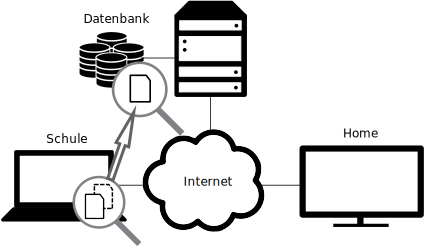
\includegraphics[]{images/dropbox_upload}
  \caption{Üblich gehandhabtes Uploaden einer Datei}
\end{figure}

Bei dem Erstellen und Bearbeiten des Übungsprotokolls auf dem Schulrechner in Form
einer Text-Datei wird eine Kopie Datei auf den vom Betreiber zur Verfügung gestellten
\gls{cloudstorage} beziehungsweise dessen Server hochgeladen und dort gespeichert.
Der Sender behält dabei die Originaldatei.

\begin{figure}[ht]
	\centering
  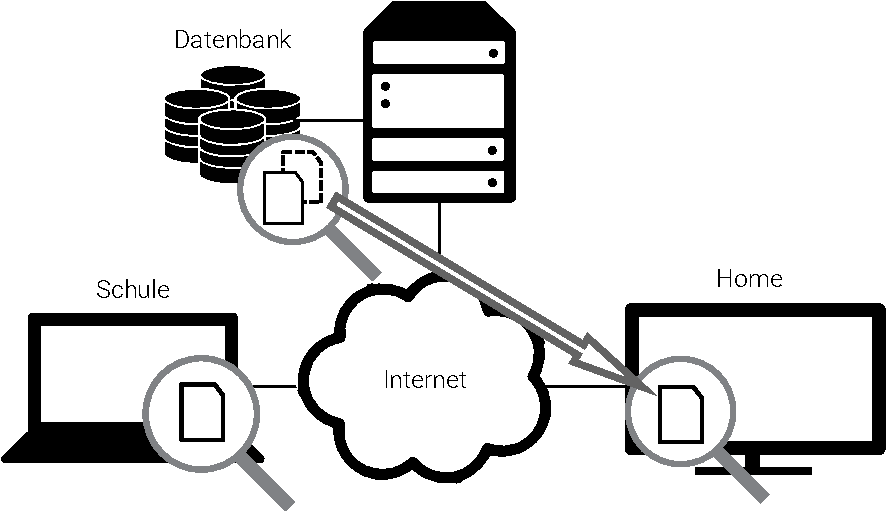
\includegraphics[]{images/dropbox_download}
  \caption{Üblich gehandhabtes Downloaden einer Datei}
\end{figure}

Wenn der Heim-PC in diesem Beispiel hochgefahren ist, wird er
über die Änderung im \gls{cloudstorage} informiert und lädt die Änderung, in
diesem Fall die neuste Version des Übungsprotokoll von dem Server herunter.
Die Text-Datei wurde somit über die zentrale Stelle, hier den Server synchronisiert.

Das Übungsprotokoll hat nach dem Synchronistationsvorgang natürlich auf dem Heim-PC
den gleichen Inhalt wie die Datei auf dem Schulrechner, da es sich um die selbe Version
handelt. Wenn man das Übungsprotokoll nun dem Heim-PC bearbeiten würde, würde
die neue Version genauso wie vorhin zuerst auf den Server geladen werden und vom Server
aus auf die einzelnen Clients, hier nur auf den Schulrechner synchronisiert
werden und die neue Version des Übungsprotokoll überschreibt die alte.

\section{Problematik}
Einen Server als Dreh- und Angelpunkt eines Dienstes einzusetzen scheint die am
einfachsten umzusetzende und kosteneffizienteste Methode zu sein, birgt aber Sicherheitsrisiken
für den Benutzer.

In der Vergangenheit kam es schon öfters zu Hackerangriffen auf große Firmen, bei
denen große Mengen an Kundendaten gestohlen wurden. Vorfälle wie diese zeigen, wie leicht
Mengen an privaten Daten in falsche Hände fallen können, wenn diese zentral an einem Ort
gespeichert werden.

Die Speicherung privater Daten von Usern auf zentralen Servern eines Unternehmens ebnet
Geheimdiensten und staatlichen Sicherheitsbehörden außerdem den Weg, flächendeckende Überwachung
durchzuführen und damit massiv in die Privatsphäre aller User des Synchronisationsdienstes
einzugreifen, da das Unternehmen als Anbieter solcher \gls{cloudstorage} unter Umständen zur
Herausgabe der Nutzerdaten gesetzlich verpflichtet ist.

% Und selbst wenn der duchschnittliche Benutzer nichts zu verbergen hat, ist der
% dreiste Eingriff in die Privatsphäre doch als äußerst problematisch einzustufen
% und leider gestaltet sich dieser zum Bedauern der betroffenen Benutzer, für
% Fremde oft viel zu einfach.
% TODO ganz umformulieren oder weglassen
Hauptursache für diese Problematik ist die unverschlüsselte und vor allem zentrale
Speicherung der Daten.

Bei \sblit werden die angesprochenen Probleme umgangen, ohne den durch Synchronisationsdienste
gebotenen Komfort zu mindern.

\section{Lösung}
\subsection{Einleitung}
Der signifikanteste Unterschied zwischen üblichen Dateisynchronisationsdiensten
und \sblit besteht im Verzicht eines Servers. Anders als im Kapitel 1.1.2. erklärt,
findet die Datenübertragung bei \sblit zwischen zwei Endgeräten nicht über einen Server statt,
sondern über eine direkte verschlüsselte Verbindung zwischen diesen zwei Geräten.

Durch diesen Ansatz fällt die zentrale Sammelstelle von Nutzerdaten
weg und dem Datendiebstahl von Hackern wird ein Riegel vorgeschoben. Außerdem
wird kein betreibendes Unternehmen mehr benötigt, um Server zu warten, womit auch
die einheitliche Anlaufstelle für staatliche Sicherheitsbehörden und Geheimdienste
nicht mehr existiert.

\subsection{Herausforderungen}
\subsubsection{Allgemein}
Mit dem Weglassen eines Servers, entstehen aber auch viele Herausforderungen,
wenn der volle Funktionsumfang eines üblichen Dateisynchronisationsdienstes
trotzdem gewährleistet werden soll.

\subsubsection{Verbindungsaufbau zwischen Clients}
So fehlt der öffentliche Server als bekannter \glqq{} Mittelmann \grqq{} in der Kommunikation
zwischen den Clients, sodass sich diese über das Internet hinwegüber mit einem
eigenen Protokoll finden, um eine direkte Verbindung erfolgreich aufbauen zu können.
Mehr zu den genauen Herausforderungen beim Verbindungsaufbau und
die Bewältigung dieser folgt später im Buch \referenz{DCL}.

\subsubsection{Alternative zu Server als \gls{filecloud}}
Der Server agiert aber nicht aber nicht nur als \glqq{} Mittelmann \grqq{} damit die
Clients miteinander kommunizieren können. Er dient nämlich auch als \gls{filecloud},
also als Zwischenspeicher für Daten. Dieser ist nämlich essenziell, wenn man
Dateien ohne große Komplikationen synchronisieren will. Um zu erklären warum das
so ist, gehen wir von folgendem Szenario bei Verwendung eines Servers aus:
Der Rechner in der Schule ist eingeschaltet, das Gerät zu Hause nicht. Wird nun
eine bereits synchronisierte Datei auf dem Schulrechner bearbeitet, wird eine Kopie dieser wie
üblich auf die \gls{filecloud}, also den Server hochgeladen. Wenn die Schule vorbei ist,
wird der Schulrechner abgedreht und zu Hause kann sofort die neuste Version der
geänderten  Datei beim Einschalten des Heim-PCs übertragen werden, obwohl der
Schulrechner ausgeschaltet ist, da die Datei in der \gls{filecloud}
zwischengespeichert wurde und sie von dort aus gesendet wurde.
\begin{figure}[h]
	\centering
  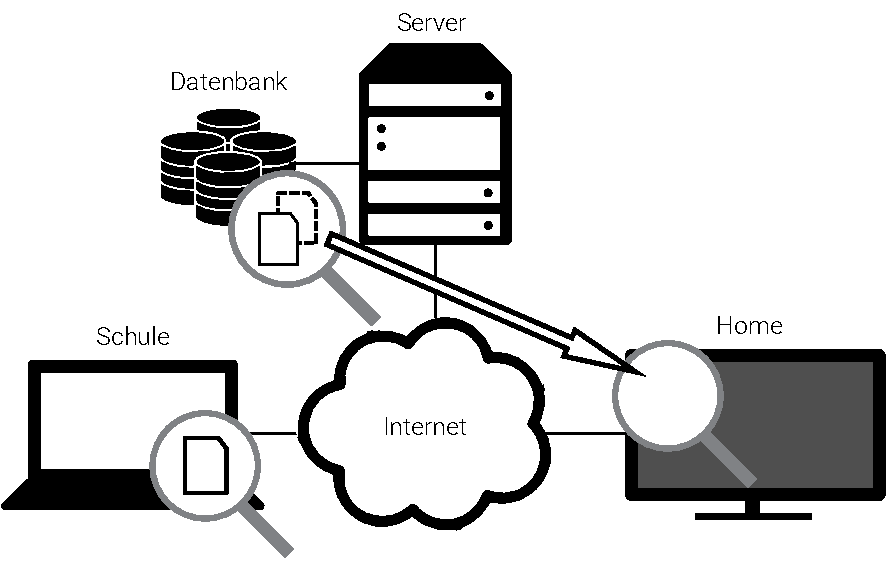
\includegraphics[]{images/dropbox_temp_1}
  \caption{Heimrechner ist nicht erreichbar. Die Datei kann nicht mit ihm
	synchronisert werden}.
\end{figure}
\begin{figure}[h]
	\centering
  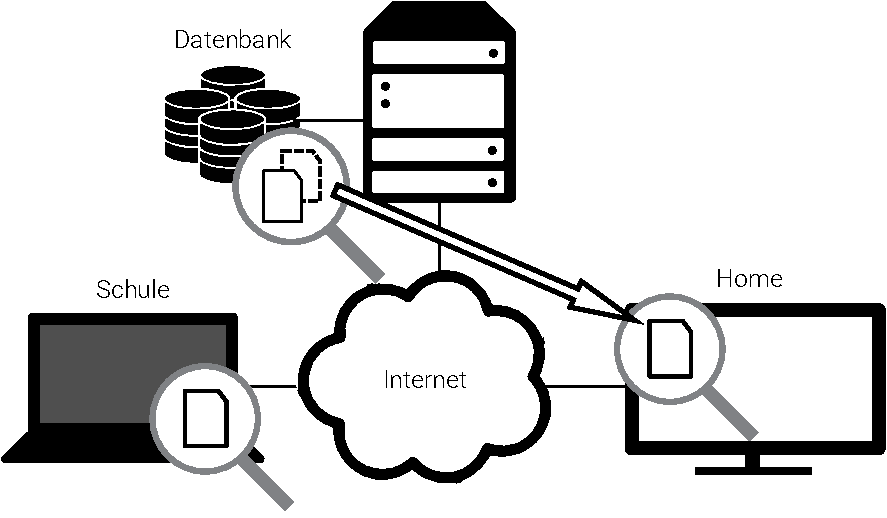
\includegraphics[]{images/dropbox_temp_2}
  \caption{Heimrechner ist wieder erreichbar, sodass die Datei nun vom Server
	bezogen werden kann}.
\end{figure}

Ohne den Server als \gls{filecloud}, wäre die alte Version der Datei bearbeitet worden, sodass zwei
neue Versionen der Datei existieren würden. Dies nennt man einen \gls{versionconflict}.
%TODO Bild einfügen, auf dem bei sblit ein Client nicht erreichbar ist.
Mit dem Verzicht auf den Server, muss also eine alternative \gls{filecloud} benutzt
werden, um Dateien zwischenspeichern zu können, sodass in vorherigen Szenario ohne Server
keine \glspl{versionconflict} auftreten.

Deshalb kommt bei \sblit eine dezentrale \gls{filecloud} zum Einsatz. Anstelle
eines zentralen Speicherns durch einen Server, wird auf den Speicherplatz der
verschiedenen Nutzern von \sblit zurückgegriffen. Diese dezentrale \gls{filecloud}
besteht also aus den verteilten Speicherplätzen verschiedenster Nutzer.

Dieses Prinzip funktioniert durch ein \gls{p2pnet}, welches durch faire Abkommen zwischen den \sblit-Nutzern realisiert wird,
sogenannten \glspl{partnership}. Grundsätzlich sind \glspl{partnership} einfach eine
Vereinbarung mit anderen, teilweise sogar fremden Nutzern, sich gegenseitig Speicherplatz
freizugeben. Eine \gls{partnership} wird entweder automatisch mit unbekannten Nutzern
geschlossen, oder durch den Nutzer selbst mit Bekannten. Genauer wird auf dieses Thema allerdings weiter hinten im Buch im
Kapitel \referenz{Partnerschaften} eingegangen.

Die Dateien werden aber natülich nicht nach einer verschlüsselten Übertragung unverschlüsselt
auf den teilweise fremden \glspl{partnerdevice} gespeichert. Verschlüsseln ist dabei
natürlich Pflicht, es wurde allerdings noch einen Schritt weiter gedacht. Generell
hat bei \sblit nämlich nur der Nutzer, dem der die Datei auf den Partnergeräten speichert und
dessen \glspl{syncpartner} Zugriff auf die vollständigen Dateien.

Wenn also mindestens ein \gls{syncpartner} nicht erreichbar ist und die Datei somit
nicht direkt über eine verschlüsselte Verbindung übertragen werden kann, wird eine Kopie
dieser Datei in viele Datenblöcke aufgeteilt. Diese Blöcke werden verschlüsselt und
verstreut auf den \glspl{partnerdevice} gespeichert.

Für die Nutzer hinter den \glspl{partnerdevice} ist es somit unmöglich auf die ursprüngliche
Datei zu schließen. Einerseits, ist der bei ihm gespeicherte Datenblock nämlich
verschlüsselt und andererseits, besitzen, wie zuvor erwähnt, nur der Nutzer, dem
der die Datei auf den Partnergeräten speichert und dessen \glspl{syncpartner}
die Information, auf welchen Geräten die verschlüsselten Datenblöcke gespeichert sind. % und in welcher Reihenfolge man diese wieder zusammensetzen muss.

Von einer ständigen Erreichbarkeit darf auch bei den \glspl{partnerdevice} nicht
ausgegangen werden. Problematisch wäre es, wenn die Datei nicht von der dezentralen
\gls{filecloud} heruntergeladen werden kann, nur weil eines von vielen \glspl{partnerdevice}
nicht erreichbar ist. Um das zu vermeiden, wird jeder verschlüsselte Datenblock so in
etwa zehn mal in der \gls{filecloud} gespeichert, sodass nur mindestens 10\% der
\glspl{partnerdevice} erreichbar sein müssen um die komplette Datei anfordern zu können.

Um den Ablauf eines Synchronisationsvorgangs bei \sblit vollständig aufzuzeigen,
folgen nun häufig auftretende Szenarios.

\subsection{Szenarios}
\subsubsection{Allgemein}
Bei \sblit wird der Inhalt eines Ordners synchronisert, der bei der
Erstinstallation der Anwendung angegebenen wurde. Sobald sich Dateien innerhalb des Ordners
ändern, wird die neue Version der Datei kopiert und die Kopie wird den
erreichbaren Synchronisationspartnern über eine direkte verschlüsselte Verbindung
gesendet.

\subsubsection{Synchronisieren zwischen zwei erreichbaren \glspl{syncpartner}}
Wenn auf dem Schulrechner eine bereits synchronisierte Datei verändert und
gespeichert wird, dann wird diese Datei in mehrere Datenblöcke
aufgeteilt, diese Blöcke werden verschlüsselt und direkt über eine verschlüsselte
Verbindung an den Heimrechner gesendet, sofern der jeweilige \gls{syncpartner}
erreichbar/eingeschalten ist. Beim \gls{syncpartner} angekommen, werden diese
entschlüsselt und zu der vollständigen neuen Datei zusammengesetzt.

\begin{figure}[h]
	\centering
  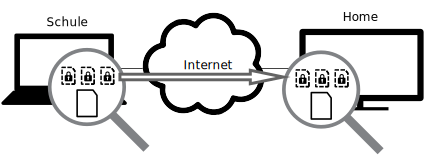
\includegraphics[]{images/sblit_p2p}
  \caption{Übertragung der Datei zwischen zwei erreichbaren Hosts}.
\end{figure}

\subsubsection{Synchronisieren zwischen zwei nicht erreichbaren \glspl{syncpartner}}
Für \glspl{syncpartner}, die nicht erreichbar sind, wird die Datei in der dezentralen
\gls{filecloud} zwischengespeichert. Die Datei wird kopiert und in Blöcke
aufgeteilt. Diese Blöcke werden verschlüsselt und verteilt auf den
\glspl{partnerdevice} gespeichert.

Da die Erreichbarkeit der gesamten Datei auf den Partnergeräten zu gewährleisten
ist, wird die Datei mehrmals
in die dezentrale \gls{filecloud} gespeichert, sodass nur ein Bruchteil der
Partnergeräte erreichbar sein muss, um auf die vollständige Datei zugreifen zu
können.

\begin{figure}[h]
	\centering
  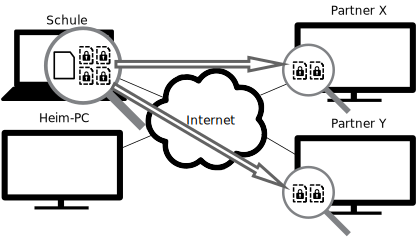
\includegraphics[]{images/sblit_upload}
  \caption{Hochladen der Datei in die dezentrale \gls{filecloud}}.
\end{figure}

Sobald der \gls{syncpartner}, hier der Heim-PC wieder hochgefahren ist, fordert er die
verschlüsselten Dateiblöcke von den \glspl{partnerdevice} an. Die Blöcke werden über
direkte verschlüsselte Verbindungen gesendet, entschlüsselt und zu der
vollständigen neuen Datei zusammengesetzt.

%Die Datei wurde somit über die aus den \glspl{partnerdevice} bestehende dezentrale
%\gls{filecloud} synchronisiert.

\begin{figure}[h]
	\centering
  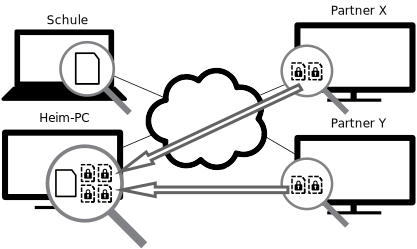
\includegraphics[]{images/sblit_download}
  \caption{Herunterladen der Datei aus der dezentralen \gls{filecloud} beziehungsweise
	den \glspl{partnerdevice}}.
\end{figure}


\chapter{Decentralized Communication Layer}
\renewcommand{\kapitelautor}{Autor: Martin Exner}

\section{Einleitung}
% TODO niemand hat besondere berechtigungen, niemand kann die funktion des netzwerks beeinträchtigen
Um die Hauptanforderung an die Umsetzung, den Verzicht auf zentrale Server im System, realisieren zu können,
wird ein \gls{p2pnet} benötigt. Über dieses läuft die Kommunikation der Synchronisationsanwendung.
Dabei muss das Netzwerk vollständig dezentral aufgebaut sein, um ohne Server funktionieren zu können.

Dieses \gls{p2pnet} ist in einer separaten \gls{cl}, \gls{dcl}, umgesetzt.
Das ermöglicht es einerseits, \gls{dcl} für Anwendungen von fremden Entwicklern zu öffnen, sodass diese auf das schon bestehende Netzwerk
zurückgreifen können und nicht erst ein eigenes umsetzen müssen, und andererseits erleichtert die klare Abgrenzung der Funktionen
zwischen \gls{cl} und eigentlicher Synchronisationsanwendung die Umsetzung beider erheblich.

\section{Anforderungen an die \gls{cl}}

Das \gls{p2pnet} des \gls{dcl} muss eine Reihe von Eigenschaften aufweisen,
um für die Anwendung eingesetzt werden zu können. Diese Eigenschaften decken sich im wesentlichen mit
üblichen Anforderungen an herkömmliche, nicht dezentrale Netzwerke und lauten wie folgt:
\begin{description}
	\item [{Adressierung:}]
		
		Den Teilnehmern müssen eindeutige Adressen zugewiesen werden können, die auf ihre Echtheit überprüfbar sind.
	
	
	\item [{Routing:}]
		
		Zwischen Teilnehmern müssen anhand ihrer Adressen Kommunikationskanäle aufgebaut werden können.

\end{description}

Durch den dezentralen Ansatz von \gls{dcl} gestaltet sich die Realisierung dieser Eigenschaften jedoch
anders als das beispielsweise für ein übliches Computernetzwerk oder das Internet der Fall wäre.
So können Adressen nicht von zentralen, dazu bemächtigten Behörden vergeben werden und das Routing
kann nicht von speziellen Teilnehmern des Netzwerks in einer hierarchischen Organisation erfolgen.



\section{Adressierung}

\subsection{Notwendigkeit}
Um in einer auf dem \gls{dcl} basierenden Anwendung Synchronisationgruppen bilden zu können, ist es
nötig, die Teilnehmer dieser Gruppen als solche erkennen zu können.
Das erfordert wiederum die permanente und eindeutige Adressierung dieser Teilnehmer.
Da sich die öffentlichen IP-Adressen der meisten privaten Internetanschlüsse und somit des Großteils der
Zielgruppe von \sblit periodisch ändern, eignen sich diese jedoch nicht als Adressen im \gls{dcl}. Es
wird also ein anderes Adresskonzept benötigt, mit dem ohne höhere Behörde allen Teilnehmern eindeutige
Adressen zugewiesen werden können, die auf ihre Echtheit überprüfbar sind.

Es ist nicht ausreichend, die Teilnehmer ihre Adressen willkürlich selbst bestimmen zu lassen und eine
Funktion zu implementieren, die überprüft, ob eine neu generierte Adresse im Netzwerk schon existiert,
da dieser Ansatz keinerlei Sicherheit vor einer absichtlichen Übernahme der Adresse eines anderen
Teilnehmers durch einen Angreifer bietet.

Dieses Unterkapitel beschreibt die Adressierung im \gls{cnet}.

% TODO schwierigkeit: keine zentrale Stelle, Eindeutigkeit

\subsection{Adressierung mit \gls*{rsa}}
\glslink{aenc}{Asymmetrische Verschlüsselungsverfahren} wie \gls{rsa} eignen sich durch ihre Eigenschaften
ausgezeichnet für die Adressierung innerhalb eines Netzwerks, in dem alle Teilnehmer die gleichen
Berechtigungen haben und in dem keine höhere Instanz existiert, die Adressen vergeben und diese
verifizieren kann.
\tags{key-info, schlüsselpaar, asymmetrisch}

Bei asymmetrischen Verschlüsselungsverfahren kommen sogenannte Schlüsselpaare, bestehend aus zwei
Schlüsseln, zum Einsatz. Die Besonderheit liegt darin, dass eine Nachricht, die mit einem Schlüssel
aus dem Schlüsselpaar verschlüsselt wurde, bei asymmetrischen Verfahren im Gegensatz zu symmetrischen
Verfahren nicht mit dem selben Schlüssel auch wieder entschlüsselt werden kann, sondern ausschließlich
mit dem anderen Schlüssel des Schlüsselpaars.
Gleichzeitig kann aus einem Schlüssel eines Schlüsselpaars der dazugehörige andere Schlüssel des
Schlüsselpaars nicht in absehbarer Zeit berechnet werden.

Dadurch wird es möglich, ein Adressierungssystem umzusetzen, das die Anforderungen im Bezug auf
Überprüfbarkeit der Adressen erfüllt. Dazu wird eine Adresse angenommen, die sich aus einem der
beiden Schlüssel aus dem Schlüsselpaar ableitet. Dieser Schlüssel wird bewusst veröffentlicht,
während der andere Schlüssel aus dem Schlüsselpaar geheim gehalten wird.
Der Schlüssel aus dem Schlüsselpaar, der veröffentlicht wird, wird auch \emph{Öffentlicher Schlüssel}
oder \emph{Public Key} genannt, der weiterhin geheim gehaltene Schlüssel \emph{Privater Schlüssel} oder
\emph{Private Key}.

Öffentliche Schlüssel als Grundlage für Adressen haben den Vorteil, dass die Adressen ohne höhere
Behörde oder zentrale Stelle auf ihre Echtheit überprüft werden können und somit fälschungssicher sind.
Ein Mechanismus zur Überprüfung solch einer Adresse wird im nächsten Abschnitt beschrieben.

\subsection{Überprüfung von Adressen}
Dadurch, dass eine mit einem öffentlichen Schlüssel verschlüsselte Nachricht nicht mit wieder mit dem
öffentlichen Schlüssel entschlüsselt werden kann, sondern ausschließlich mit dem dazugehörigen privaten
Schlüssel, kann der Besitz des gesamten Schlüsselpaars bewiesen werden, ohne mehr als den öffentlichen
Schlüssel preisgeben zu müssen: Eine beliebige Folge von Daten wird vom überprüfenden Teilnehmer
generiert, mit der Grundlage der Adresse des zu überprüfenden Teilnehmers, also seinem öffentlichen
Schlüssel verschlüsselt und anschließend an diesen übermittelt. Dort wird die empfangene Nachricht vom zu
überprüfenden Teilnehmer mit seinem privaten Schlüssel, den nur dieser Teilnehmer besitzt, wieder
entschlüsselt und zurück an den überprüfenden Teilnehmer gesendet.

Decken sich die ursprünglich vom überprüfenden Teilnehmer generierten Daten mit denen, die vom zu
überprüfenden Teilnehmer entschlüsselt wurden, ist der Besitz des gesamten Schlüsselpaars, und nicht
lediglich des öffentlichen Schlüssels, bewiesen. In anderen Worten, die vom überprüften Teilnehmer
bekanntgegebene Adresse ist echt.

%TODO konkretes Beispiel

%TODO Erklärung der Challenge mit Nikolas mergen

\subsection{Eindeutigkeit von Adressen}
\label{dcl-addr-uniqueness}
Die Eindeutigkeit der generierten \gls{rsa}-Schlüsselpaare und somit der Adressen kann zwar nicht
garantiert werden, eine Kollision ist jedoch aufgrund der Länge der verwendeten Schlüssel und der
Anzahl der dadurch möglichen Schlüsselpaare dermaßen unwahrscheinlich, dass davon ausgegangen
werden kann, dass eine Kollision praktisch nicht auftritt. \cite{crypto.stackexchange.com/a/2559:rsa-key-collision}

\subsection{Adressformat}

\subsubsection{\gls*{rsa}-Schlüssellänge}
Die für die Adressen im \gls{dcl} verwendeten öffentlichen \gls{rsa}-Schlüssel haben eine Länge von \addrkeybits
Bits, was \addrkeybytes Bytes entspricht.
IPv4 und IPv6-Adressen haben mit jeweils 32 Bits (4 Bytes) bzw. 128 Bits (16 Bytes) vergleichsweise kurze
Adressen. Trotzdem ist eine Adressierung mit 128 Bits mehr als ausreichend und wesentlich längere
Adressen, wie sie beispielsweise bei direkter Verwendung von RSA-Schlüsseln entstehen, bringen
lediglich Nachteile und keinerlei Vorteile mit sich, da der dabei entstehende Overhead bei Nachrichten
eine wesentliche Reduktion der Übertragungseffizienz mit sich bringt.

\subsubsection{Adressverkürzung}
Die im \gls{dcl} verwendeten Adressen decken sich nicht mit den öffentlichen \gls{rsa}-Schlüsseln,
sondern basieren lediglich darauf. Da ohne Weiterverarbeitung der Schlüssel zu lange Adressen entstünden,
wird auf die Daten der öffentlichen Schlüssel ein \gls{hash} angewandt, welcher die Daten in einem ersten
Schritt wesentlich verkürzt. In einem optionalen zweiten Schritt können die bereits verkürzten
Daten weiter verkürzt werden, um unnötig lange Adressen zu eliminieren.

Nachfolgend ist jener Teil des Quellcodes von \gls{dcl} angeführt, welcher im \code{\gls{cnt}}
zur Adressverkürzung angewandt wird.

\javalisting
\begin{minipage}{\linewidth}
\begin{lstlisting}[caption={Adressverkürzung im \gls*{cnt} (Java)},captionpos=b]
Data scaleAddress(Address address) {
	
	Data fullData = address.toData();
	Data hashedData = hash.update(fullData).finish();
	
	if(byteLength == hashedData.length()) return hashedData;
	
	Data scaledData = new Data(byteLength);
	
	for(int i = 0; i < hashedData.length(); i++) {
		int scaledIndex = i % scaledData.length();
		scaledData.setByte(
			scaledIndex,
			(byte)( scaledData.getByte(scaledIndex)
					^ hashedData.getByte(i))
		);
	}
	
	return scaledData;
	
}
\end{lstlisting}
\end{minipage}

\begin{description}
	
	\descriptionitem{\code{address}}
		Das \javaarg \code{address} referenziert ein \code{\gls{Address}}-Objekt, welches den
		als Grundlage für eine Adresse verwendeten öffentlichen Schlüssel enthält.
	
	\descriptionitem{\code{\gls{Data}}}
		\glsdesc{Data}.
	
	\descriptionitem{\code{hash}}
		Die \javainstvar \code{hash} referenziert ein \code{\gls{Hash}}-Objekt, welches den
		im \gls{nt} angegebenen \gls{hash} implementiert.
	
	\descriptionitem{\code{byteLength}}
		Die \javainstvar \code{byteLength} enthält die Ziellänge der Adressen, in bytes.
	
\end{description}

Mit \code{address.toData()} wird der öffentliche Schlüssel der übergebenen Adresse zuerst in Binärdaten
umgewandelt, auf welche dann ein \gls{hash} angewandt wird. Entspricht die Ziellänge von Adressen im
\gls{nt} der \gls{digestlength} des verwendeten \gls{hash}, so wird der \gls{hashval} \code{hashedData}
direkt zurückgegeben.

Anderenfalls wird der \gls{hashval} aus \code{hashedData} auf Binärdaten der Länge \code{byteLength},
gespeichert in \code{scaledData}, abgebildet und diese zurückgegeben.




\chapter{Sblit}
\renewcommand{\kapitelautor}{Autor: Nikola Szucsich}

\section{Kommunikation}\label{kommunikation}
Um zu verhindern, dass Daten mitgelesen werden, verwendet \sblit den sicheren \nameref{Applicationchannel} (siehe Seite \pageref{Applicationchannel}) der Kommunikationsschicht.\\
\sblitg verwendet zur Kommunikation fünf verschiedene Nachrichten:
\begin{itemize}
	\item Authentifizierungsanfragen
	\item Antworten auf Authentifizierungsanfragen
	\item Dateianfragen
	\item Antworten auf Dateianfragen
	\item Die eigentliche Übertragung der Datei
	\item Löschanfragen
\end{itemize}
\subsection{\gls{authreq}}
Angenommen zwei Geräte eines Besitzers wollen Daten austauschen. Wie können sich diese sicher sein, dass es sich auch um das richtige Gerät handelt? Hier kommt die Authentifizierung ins Spiel. \gls{authreq}s dienen zur Sicherstellung der Authentizität des Gerätes (im Folgenden Gerät A), mit dem ein anderes Gerät (im Folgenden Gerät B) eine Verbindung aufbaut. Dazu schickt das Gerät B zufällige Daten an Gerät A mit der Aufforderung, diese zu verschlüsseln. Die Nachricht ist dabei folgendermaßen aufgebaut:
\begin{figure}[H]
\begin{centering}

\begin{bytefield}[bitwidth=3em]{8}
	\\
	\bitheader{0-7} \\
	
	\begin{rightwordgroup}{\isprotomsgtype}
		\wordbox[tlr]{1}{0}
	\end{rightwordgroup} \\
	
	\begin{rightwordgroup}{\isprotomsgdata}
		\wordbox[tblr]{4}{Zufallsdaten, 64 Bytes} 
	\end{rightwordgroup}
	
\end{bytefield}

\par\end{centering}
\protect\caption{\gls{authreq}}
\end{figure}
%TODO Umformulieren
Die Gesamtlänge der Daten, die mit RSA-2048 verschlüsselt werden, darf maximal 128 Byte lang sein. Um Gerät A 64 Byte zur Verfügung zu stellen, beträgt die Länge der von Gerät B gesendeten Daten 64 Byte. Diese 64 Byte werden von Gerät A benötigt, um zu verhindern, dass Gerät B sich gewünschte Werte von Gerät A verschlüsseln lässt.

\subsection{\gls{authres}}
Bevor die Daten wieder zurückgeschickt werden, müssen diese von Gerät B verschlüsselt werden. Dies geschieht mit dem Private-Key des Gerätes B. Dabei wird vorher noch ein zufälliger Wert an die empfangenen Daten angefügt, um das unter Authentifizierungsanfragen beschriebene Problem zu lösen.\\
Der Aufbau der Nachricht lautet wie folgt:
\begin{figure}[H]
\begin{centering}

\begin{bytefield}[bitwidth=3em]{8}
	\\
	\bitheader{0-7} \\
	
	\begin{rightwordgroup}{\isprotomsgtype}
		\wordbox[tlr]{1}{1}
	\end{rightwordgroup} \\
	
	\begin{rightwordgroup}{\isprotomsgdata}
		\wordbox[tblr]{4}{Verschlüsselte Daten, 128 Bytes} 
	\end{rightwordgroup}
	
\end{bytefield}

\par\end{centering}
\protect\caption{\gls{authres}}
\end{figure}
Wird dieses Paket nun von Gerät B empfangen, kann der Inhalt mit dem Public-Key des Gerätes A, also dessen Adresse, entschlüsselt werden. Von den erhaltenen Daten werden die ersten 64 Byte mit den ursprünglich gesendeten 64 Byte verglichen. Stimmen die beiden Werte überein, kann das Gerät seine Authentizität beweisen. Stimmen diese jedoch nicht überein, handelt es sich um einen Betrüger, der offensichtlich den richtigen Private-Key zur von ihm angegebenen Adresse nicht kennt.
		
\subsection{\gls{filereq}} \label{Dateianfrage}
Bevor eine Datei an ein anderes Gerät (im Folgenden Gerät B) verschickt wird, schickt das Gerät, das die Datei besitzt (im Folgenden Gerät A), eine Dateianfrage an das Gerät B. Dies hat 2 Gründe: Erstens muss eruiert werden, ob die Datei überhaupt von Gerät B benötigt wird, oder ob besagtes Gerät schon diese Datei besitzt. Zweitens besteht die Möglichkeit eines Konfliktes \referenz{Konflikt}. Daher ist die Dateianfrage folgendermaßen aufgebaut:
\begin{figure}[H]
\begin{centering}

\begin{bytefield}[bitwidth=3em]{8}
	\\
	\bitheader{0-7} \\
	
	\begin{rightwordgroup}{\isprotomsgtype}
		\wordbox[tlr]{1}{2}
	\end{rightwordgroup} \\
	
	\begin{rightwordgroup}{\isprotomsgdata}
		\wordbox[tlr]{2}{Dateipfad, variable Länge} \\
		\skippedwords \\
		\wordbox[lr]{1}{} \\
		\wordbox[tlr]{2}{Versionsverlauf, variable Länge} \\
		\skippedwords \\
		\wordbox[blr]{1}{}
	\end{rightwordgroup}
	
\end{bytefield}
\par\end{centering}
\protect\caption{\gls{filereq}}
\end{figure}
\begin{description} 
	\item[{Dateipfad}] \hfill \\
		Hierbei wird der zu \sblit's Hauptordner relative Dateipfad mitgeschickt. Der absolute Dateipfad wird aus dem Grund nicht mitgeschickt, da der Ort des \sblit-Ordners nicht auf allen Geräten gleich sein muss. Befindet sich der Ordner auf Gerät A beispielsweise unter C:/Users/Susanne/ kann sich der Ordner auf Gerät B auch unter /home/susanne/dateien/ befinden.
	\item[{Versionsverlauf}] \hfill \\
		Der Versionsverlauf beinhaltet alle Hashes einer Datei seit der letzten komplett synchronisierten Version. Das heißt, dass auf jedem Gerät aktuell entweder diese oder eine neuere Version gespeichert ist.
\end{description}

		
\subsection{\gls{fileres}}
Die Antwort auf eine Dateianfrage beinhaltet folgende Parameter: 

\begin{figure}[H]
\begin{centering}

\begin{bytefield}[bitwidth=3em]{8}
	\\
	\bitheader{0-7} \\
	
	\begin{rightwordgroup}{\isprotomsgtype}
		\wordbox[tlr]{1}{3}
	\end{rightwordgroup} \\
	
	\begin{rightwordgroup}{\isprotomsgdata}
		\wordbox[tlr]{1}{Need-Flag, 1 Byte} \\
		\wordbox[tlr]{2}{Dateipfad, variable Länge} \\
		\skippedwords \\
		\wordbox[lr]{1}{} \\
		\wordbox[tlr]{2}{Hash, variable Länge} \\
		\skippedwords \\
		\wordbox[blr]{1}{}
	\end{rightwordgroup}
	
\end{bytefield}
\par\end{centering}
\protect\caption{\gls{fileres}}
\end{figure}

\begin{description}
	\item[{Need-Flag}] \hfill \\
		Dieses Feld enthält einen Hexadezimalwert, der darüber Auskunft gibt, ob die Datei benötigt wird oder nicht. Steht in diesem Feld der Hexadezimalwert 0x00, wird die Datei nicht benötigt. Steht hier hingegen der Hexadezimalwert 0x01, wird die Datei benötigt. Dieses Byte hilft den Datenverkehr zu reduzieren. So muss nicht eine ganze Datei verschickt werden muss, obwohl diese gar nicht gebraucht wird.
	\item[{Dateipfad}] \hfill \\
		Wie auch bei der Dateianfrage wird in der Antwort auf die Dateianfrage der zu \sblit's Hauptordner relative Pfad mitgeschickt.
	\item[{Hash}] \hfill \\
		Hier wird noch einmal der letzte Hash des Versionsverlaufs der Dateianfrage verschickt, um sicherzustellen, dass die Datei in der Zwischenzeit nicht geändert wurde. 
\end{description}
Nach Empfang der Dateianfrage wird zunächst geprüft, ob die Datei vorhanden und in der aktuellst ist.  Ist die lokale Datei nicht aktuell, wird das Need-Flag, auf den Hexadezimalwert 0x01 gesetzt. Ist die Datei auf dem aktuellsten Stand, wird besagtes Flag auf den Hexadezimalwert 0x00 gesetzt. Außerdem wird überprüft, ob ein Konflikt aufgetreten ist \referenz{Konflikterkennung}.\\
Nach Empfang der Antwort wird zunächst überprüft, ob der Hashwert der Datei mit dem erhaltenen Pfad übereinstimmt. Stimmt der Hashwert in der Anfrage nicht mit dem aktuellen Hashwert überein, wird die Antwort verworfen. Dies kann beispielsweise passieren, wenn in der Zwischenzeit eine neuere Version der Datei erzeugt wurde. Stimmt dieser jedoch überein, kann die Datei nun im nächsten Schritt verschickt werden.
		
\subsection{Die eigentliche Übertragung der Datei}
Bei der eigentlichen Übertragung der Datei werden folgenden Daten mit der Datei mitgesendet: 
\begin{figure}[H]
\begin{centering}

\begin{bytefield}[bitwidth=3em]{8}
	\\
	\bitheader{0-7} \\
	
	\begin{rightwordgroup}{\isprotomsgtype}
		\wordbox[tlr]{1}{5}
	\end{rightwordgroup} \\
	
	\begin{rightwordgroup}{\isprotomsgdata}
		\wordbox[tlr]{2}{Dateiinhalt, variable Länge} \\
		\skippedwords \\
		\wordbox[lr]{1}{} \\
		\wordbox[tlr]{2}{Dateipfad, variable Länge} \\
		\skippedwords \\
		\wordbox[lr]{1}{} \\
		\wordbox[tlr]{2}{Hashes, variable Länge} \\
		\skippedwords \\
		\wordbox[lr]{1}{} \\
		\wordbox[tlr]{2}{Geräte mit der aktuellen Verision, variable Länge} \\
		\skippedwords \\
		\wordbox[blr]{1}{}
	\end{rightwordgroup}
	
\end{bytefield}
\par\end{centering}
\protect\caption{\gls{filemsg}}
\end{figure}

\begin{description}
	\item[{Dateiinhalt}] \hfill \\
		Der Dateiinhalt wird als binäres \code{Data}-Objekt verschickt.
	\item[{Geräte mit der aktuellen Version}] \hfill \\
		Hier stehen die Adressen aller Geräte, die die neuste Version schon haben. Ist die Version auf allen Geräten aktuell, kann diese von den Partnergeräten gelöscht werden. Daher wird diese Liste an Geräten immer mit der Datei mitgeschickt. Außerdem können somit unnötige Anfragen an Geräte, die die Datei schon besitzen verhindert werden.
	\item[{Dateipfad}] \hfill \\
		Der Dateipfad wird benötigt, damit die Datei auf dem zu synchronisierenden Gerät weiß, an welchen Ort die Datei gespeichert werden soll. Dies ist der gleiche relative Ort, wie auf dem Gerät, das die Anfrage geschickt hat.
	\item[{Hashes}] \hfill \\
		Die Hashes werden mitgeschickt, um einen einheitlichen Versionsverlauf sicherzustellen. Das verhindert das auftreten von Konflikten, welche gar keine sind. Weiters dient der aktuellste Hash dazu,  sicherzustellen, dass die Datei, die versendet wurde, auch so ankommt, wie sie versendet wurde. Verhasht man die neue Datei, muss das Ergebnis mit dem aktuellsten mitgeschickten Hash übereinstimmen. Andernfalls muss die Datei neu gesendet werden.
\end{description}
		
\subsection{Löschanfrage}
\begin{figure}[H]
\begin{centering}

\begin{bytefield}[bitwidth=3em]{8}
	\\
	\bitheader{0-7} \\
	
	\begin{rightwordgroup}{\isprotomsgtype}
		\wordbox[tlr]{1}{5}
	\end{rightwordgroup} \\
	
	\begin{rightwordgroup}{\isprotomsgdata}
		\wordbox[tlr]{2}{Dateipfad, variable Länge} \\
		\skippedwords \\
		\wordbox[blr]{1}{} \\
	\end{rightwordgroup}
	
\end{bytefield}
\par\end{centering}
\protect\caption{\gls{filemsg}}
\end{figure}		
Eine Löschanfrage beinhaltet den Pfad der zu löschenden Datei. Nach Empfang der Löschanfrage wird die Datei gelöscht.



\section{Datei-Verarbeitung}\label{dateiverarbeitung}
\subsection{Allgemein}
Ein wesentlicher Bestandteil von \sblit ist die Verarbeitung der Dateien. Dazu zählen das Erkennen von Änderungen sowie das Erkennen und Lösen von Konflikten.
\subsection{Versionierung}\label{Logfile}
Ein wichtiges Mittel zur Verwaltung der Dateien ist das \gls{logfile}. Dieses enthält Informationen zu allen Dateien im \sblit-Ordner. Dazu zählen der relative Dateipfad, eine Liste mit Hashes, die für die Versionierung zuständig sind, und eine Liste an Geräten, auf denen die Datei bereits auf dem aktuellen Stand ist. Weiters wird in dieser Datei festgehalten, ob Dateien im Konflikt zu anderen Dateien stehen. Die Versionierung ist vor allem für die Konflikterkennung \referenz{Konflikterkennung} notwendig. Hierbei werden Hashes für alle Versionen der Dateien gespeichert. Die Version wird beim Speichern der Datei um den aktuellen Hashwert erweitert und bei Konvergenz auf allen Geräten auf die aktuelle gemeinsame Version reduziert. 

Damit \sblit weiß, wann die Dateien von den Partnergeräten \referenz{Partnergerät} wieder gelöscht werden können, wird eine Liste von Geräten, mit Dateien auf dem aktuellen Stand, gespeichert. Diese Liste wird bei jeder Änderung mit der Liste aller eigenen Geräte verglichen. Sobald alle eigenen Geräte eingetragen sind, werden die Partnergeräte aufgefordert, die Datei zu löschen. 

\subsection{Reaktionen auf Dateiänderungen}
Wenn eine Datei neu erstellt, bearbeitet oder gelöscht wird, erkennt dies \sblit und leitet diese Informationen an den Synchronisationsprozess weiter. Außerdem ist das Erkennen einer Änderung im \sblit-Ordner wichtig, damit sie im \gls{logfile} protokolliert werden kann. Das \gls{logfile} wird sowohl für die Konflikterkennung \referenz{Konflikterkennung} als auch für die Reduktion der benötigten Bandbreite \referenz{Dateianfrage} genutzt.

Um Änderungen zu erkennen, verwendet \sblit das sogenannte \gls{watchservice}. Das \gls{watchservice} wird bei Änderungen in dem Ordner, der vom Benutzer für die Synchronisation festgelegt wurde, benachrichtigt. Je nach dem, ob eine Datei angelegt, verändert oder gelöscht wurde, erfolgen unterschiedliche Arbeitsschritte. Beim Anlegen einer neuen Datei, wird ihr Pfad samt Hash in das \gls{logfile} geschrieben und eine Dateianfrage an die anderen eigenen Geräte geschickt. Wird eine Datei verändert, wird ein neuer Hash zu den bereits vorhandenen Hashes hinzugefügt. Außerdem wird eine Dateianfrage an die anderen eigenen Geräte gesendet. Wird eine Datei gelöscht, wird sie samt Hashes aus dem \gls{logfile} entfernt. Anschließend wird eine Löschanfrage an die eigenen Geräte versandt.\\ \\
\listingstart{Initialisierung des \gls{watchservice}}
WatchService watcher = filesDirectory.getFileSystem()
		.newWatchService();
filesDirectory.register(watcher,
		StandardWatchEventKinds.ENTRY_CREATE,
		StandardWatchEventKinds.ENTRY_DELETE,
		StandardWatchEventKinds.ENTRY_MODIFY);
WatchKey watchKey = watcher.take();
List<WatchEvent<?>> events = watchKey.pollEvents();
Thread.sleep(TIME_TO_SLEEP);
Map<String, LinkedList<Data>> logs = getLogs();
Map<String, LinkedList<Data>> synchronizedDevices = 
		getSynchronizedDevices();
\end{lstlisting}
\begin{description}
	\descriptionitem{filesDirectory}
	\code{filesDirectory} enthält den vom Benutzer festgelegten \sblit-Ordner.
	\descriptionitem{watcher}
	\code{watcher} wird benötigt, um das \gls{watchservice} einen bestimmten Ordner überwachen zu lassen.
	\descriptionitem{watchKey}
	\gls{watchkey} enthält eine Liste an Dateien, die neu erstellt, geändert oder gelöscht wurden.
	\descriptionitem{events}
	Jedes \code{WatchEvent} aus der \code{List events} enthält eine Datei, die sich geändert hat und die Information, ob sie neu erstellt, verändert oder gelöscht wurde. 
	\descriptionitem{logs}
	\code{logs} enthält den Versionsverlauf aller Dateien, die sich im \sblit-Ordner befinden.
	\descriptionitem{synchronizedDevices}
	\code{synchronizedDevices} enthält zu jeder Datei eine Liste an Geräten, auf denen die akuelle Version gespeichert ist.
\end{description}
Zunächst wird ein neues Objekt vom Typ \code{\gls{watchservice}} erstellt. Dieses überwacht den festgelegten \sblit-Ordner hinsichtlich neu erstellter, geänderter und gelöschter Dateien. Zur Registrierung des \gls{watchservice} im Dateisystem, werden in der \code{register}-Methode das \gls{watchservice}-Objekt und die Fälle, in denen das \gls{watchservice} benachrichtigt werden soll, festgelegt. In diesem Fall ist sind das neue Dateien (\code{ENTRY\_CREATE}), Dateiänderungen (\code{ENTRY\_MODIFY}) und gelöschte Dateien (\code{ENTRY\_DELETE}). Die \code{take}-Methode wartet auf Änderungen im festgelegten Ordner und übergibt sie dann an das \code{\gls{watchkey}}-Objekt. Die Anweisung \code{watchKey.pollEvents()} unterteilt den \gls{watchkey} in einzelne Dateiänderungen und formatiert diese für den weiteren Gebrauch. 

Der Thread wird angehalten, da das Programm beim Empfangen einer Datei das Logfile bearbeitet. Dies passiert, damit \sblit weiß, dass die Datei nicht vom Nutzer verändert wurde. \\ \\
\listingstart{Unterteilen in einzelne Dateien}
for (WatchEvent event : events) {
	String path = event.context().toString();
	File changedFile = new File(
			Configuration.getSblitDirectory()
					+ Configuration.slash + path);
\end{lstlisting}
\begin{description}
	\descriptionitem{event}
	\code{event} enthält Informationen zur Erstellung, Änderung oder Bearbeitung einer Datei aus der Liste \code{events}. 
	\descriptionitem{path}
	\code{path} enthält den relativen Pfad zur geänderten Datei.
	\descriptionitem{changedFile}
	\code{changedFile} enthält die Datei, die gerade geändert wurde.
\end{description}
\listingstart{Erstellen einer Datei}
if (event.kind() == StandardWatchEventKinds.ENTRY_CREATE 
		&& logs.get(path) == null) {
	byte[] fileContent = 
			Files.readAllBytes(changedFile.toPath());
	Data hash = Crypto.sha1(new Data(fileContent));
	LinkedList<Data> hashes = new LinkedList<>();
	hashes.add(hash);
	logs.put(path, hashes);
	LinkedList<Data> devices = new LinkedList<>();
	devices.add(Configuration
			.getPublicAddressKey().toData());
	synchronizedDevices.put(path, devices);
	filesToPush = refreshFilesArray(filesToPush, changedFile);
}
\end{lstlisting}
\begin{description}
	\descriptionitem{fileContent}
	\code{fileContent} enthält den Inhalt der Datei, die neu erstellt wurde.
	\descriptionitem{hash}
	In \code{hash} wird der Hashwert des Inhalts der Datei gespeichert.
	\descriptionitem{hashes}
	\code{hashes} enthält den Versionsverlauf einer Datei. 
	\descriptionitem{devices}
	\code{devices} enthält alle Geräte, auf denen die Datei aktuell ist. In diesem Fall ist das genau das Gerät, auf dem der Code ausgeführt wird, da diese Datei gerade erst erstellt wurde.
\end{description}
Wenn eine Datei erstellt wurde, wird sie zu allererst ausgelesen. Anschließend wird der Inhalt verhasht und dem Versionverlauf hinzugefügt. Außerdem wird das Gerät, auf dem der Code ausgeführt wird, zur Geräteliste \code{devices} hinzugefügt. Schließlich wird die Datei zur Liste der zu synchronisierenden Dateien hinzugefügt.\\ \\
\listingstart{Löschen einer Datei}
else if (event.kind() == StandardWatchEventKinds
		.ENTRY_DELETE) {
	logs.remove(path);
	synchronizedDevices.remove(path);
	filesToDelete = refreshFilesArray(filesToDelete,
			changedFile);
}
\end{lstlisting}
Beim Löschen einer Datei wird der zugehörige Versionsverlauf ebenfalls entfernt. Außerdem wird der Variable \code{filesToDelete} der Pfad der gelöschten Datei hinzugefügt, um die anderen eigenen Geräte auch darüber zu informieren, dass eine Datei gelöscht wurde. \\ \\
\listingstart{Bearbeiten einer Datei}
else if (event.kind() == StandardWatchEventKinds
		.ENTRY_MODIFY) {
	byte[] fileContent = readFile(event);
	Data hash = Crypto.sha1(new Data(fileContent));
	LinkedList<Data> hashes = logs.get(path);
	if (!hashes.contains(hash)) {
		hashes.add(hash);
		filesToPush = refreshFilesArray(filesToPush,
				changedFile);
		LinkedList<Data> devices = new LinkedList<>();
		devices.add(Configuration
				.getPublicAddressKey().toData());
		synchronizedDevices.put(path, devices);
	}
}
\end{lstlisting}
\begin{description}
\descriptionitem{fileContent}
	\code{fileContent} enthält den Inhalt der Datei, die bearbeitet wurde.
	\descriptionitem{hash}
	In \code{hash} wird der Hashwert des Inhalts der Datei gespeichert.
	\descriptionitem{hashes}
	\code{hashes} enthält den Versionsverlauf der Datei. 
	\descriptionitem{devices}
	\code{devices} enthält alle Geräte, auf denen die Datei aktuell ist. In diesem Fall ist das genau jenes Gerät, auf dem der Code ausgeführt wird, da diese Datei gerade bearbeitet wurde.
\end{description}
Wurde die Datei bearbeitet, wird sie ausgelesen und anschließend verhasht. Nachdem der Versionsverlauf für die Datei in der Variable \code{hashes} gespeichert wurde, wird überprüft, ob der Versionsverlauf die Datei schon enthält. Ist dies der Fall, ist ein Fehler aufgetreten und die neue Version wird nicht synchronisiert. Falls der Versionsverlauf die aktuelle Version noch nicht enthält, wird der Hash der aktuellen Version im Versionsverlauf gespeichert. Anschließend wird eine neue Liste an Geräten erstellt, auf denen schon die neuste Version synchronisiert ist. In diesem Fall wird nur das eigene Gerät hinzugefügt, da die neuste Version bis jetzt nur auf diesem Gerät vorhanden ist. \\ \\
\listingstart{Schreiben des \gls{logfile}s}
}
logFile.createNewFile();
write(files, synchronizedDevices);
\end{lstlisting}
Das \gls{logfile} wird neu erstellt und die neuen Daten werden anschließend darin gespeichert.
\subsection{Konflikte}\label{Konflikt}
\subsubsection{Allgemein}
Ein Konflikt ist ein Problem, das bei Synchronisationsdiensten vorkommt. Dieser tritt auf, wenn eine Datei bearbeitet wird, bevor sie synchronisiert werden kann. 

Dazu ein Beispiel: Susanne hat einen Laptop und einen Stand-Rechner, auf denen sie mithilfe von \sblit einen Ordner synchronisiert. Im Normalfall, also wenn kein Konflikt auftritt, bearbeitet Susanne eine Datei auf dem Laptop. Nach dem Speichern wird die Datei auf den Stand-Rechner übertragen und dort gespeichert. Die Datei ist nun auf beiden Geräten synchron.

Angenommen, Susanne schaltet nun den Laptop aus und bearbeitet anschließend die Datei noch einmal auf dem Stand-Rechner. Da der Laptop ausgeschaltet ist, kann die Datei nicht synchronisiert werden. Auf dem Weg zur Arbeit fällt Susanne noch eine Verbesserungsmöglichkeit der Datei ein und sie bearbeitet die Datei auf dem Laptop ohne einer Verbindung zum Internet. In der Arbeit angekommen, packt Susanne wieder ihren Laptop aus und verbindet sich zum Internet. Die Datei kann jetzt nicht auf den neusten Stand gebracht werden, da ja zwei unterschiedliche Versionen existieren. Würde die Datei einfach vom Stand-Rechner auf den Laptop kopiert werden, gingen die Neuerungen am Laptop verloren, umgekehrt würde die Datei vom Laptop die Änderungen am Stand-Rechner überschreiben. Diesen Zustand zweier verschiedener Versionen der gleichen Datei, ohne die Änderungen des jeweils anderen Gerätes schon berücksichtigt zu haben, nennt man einen Konflikt.
%TODO eventuell noch ergänzen

\subsubsection{Konflikterkennung}\label{Konflikterkennung}
Um Konflikte zu erkennen, verwendet \sblit eine interne Versionierung der Dateien. Diese wird im Kapitel \linkt{Logfile} näher erklärt. Bei einer Dateianfrage \referenz{Dateianfrage} werden alle Hashes einer Datei mitgesendet. Diese werden nach dem Empfang der Anfrage mit den Hashes der Datei mit dem gleichen Namen und aller Konfliktdateien dieser Datei im lokalen \gls{logfile} verglichen. Stimmen die beiden aktullen Hashes aus Dateianfrage und der Datei mit dem gleichen Namen im \gls{logfile} überein, muss die Datei gar nicht übertragen werden, da sie schon auf dem neusten Stand ist. Das heißt natürlich auch, dass kein Konflikt auftritt. Stimmt der aktuelle Hash im lokalen \gls{logfile} mit einem in der Dateianfrage überein, tritt ebenfalls kein Konflikt auf, da der aktuelle lokale Hash dem Gerät, das die Anfrage verschickt hat, schon bekannt ist. 

Stimmt der Versionsverlauf aus dem \gls{filereq} mit dem einer Konfliktdatei überein, wurde eine Version synchronisiert, bevor ein drittes Gerät einen Konflikt bemerkt hat. In diesem Falle könnten mehrere Konfliktdateien mit nur zwei verschiedenen Inhalten erstellt werden. Passiert dies, werden die Namen der beiden Dateien vertauscht, um das eben genannte Szenario zu verhindern.

Ist der aktuelle Hash der lokalen Datei jedoch nicht in der Dateianfrage enthalten, wurde die lokale Datei bearbeitet, bevor diese auf den aktuellsten Stand gebracht werden konnte. Anders gesagt: Ein Konflikt ist aufgetreten.

\subsubsection{Konfliktlösung}
Damit die Änderungen von einem Gerät nicht überschrieben werden, speichert \sblit beide Versionen. Da jedoch beide Dateien nicht den gleichen Namen haben können, benennt das Gerät, das den Konflikt erkennt, (im Folgenden Gerät A) die lokale Datei um. Anschließend schickt Gerät A eine Antwort an das Gerät, das die Dateianfrage geschickt hat,  (im Folgenden Gerät B) in der es die neue Version anfordert, als ob kein Konflikt aufgetreten wäre. Außerdem schickt Gerät A eine Dateianfrage mit der neuen Datei an Gerät B. Gerät B sendet nun die angeforderte Datei an Gerät A und akzeptiert die Konfliktdatei, da es eine Datei mit dem gleichen Namen noch nicht besitzt. 

Nach dem Empfang der Datei speichtert Gerät A diese unter dem ursprünglichen Namen. Des Weiteren sendet Gerät A die Konfliktdatei mit dem geänderten Namen an Gerät B. Die neue Datei wird auf Gerät B unter dem neuen Namen gespeichert.

\subsubsection{Umsetzung}
Um Konflikte zu erkennen und zu lösen wird der folgende Code verwendet: \\ \\
\listingstart{Erkennen eines Konflikts}
private void handleConflict(LinkedList<Data> requestedHashes, LinkedList<Data> ownHashes, String path) throws IOException {
	String sblitDirectory = Configuration.getSblitDirectory() + Configuration.slash;
	if (!requestedHashes.contains(ownHashes.get(ownHashes.size() - 1))) {
		int dotIndex = path.lastIndexOf(".");
		File conflictFile;
		if (dotIndex > path.lastIndexOf(Configuration.slash) + 1) {
			for (int i = 1;; i++) {
				conflictFile = new File(sblitDirectory + path.substring(0, dotIndex) + "(Conflict " + i + ")" + path.substring(dotIndex));
				if (!conflictFile.exists()) {
					break;
				}
			}
		} else {
			for (int i = 1;; i++) {
				conflictFile = new File(sblitDirectory + path
						+ "(Conflict " + i + ")");
				if (!conflictFile.exists()) {
					break;
				}
			}
		}
		File file = new File(sblitDirectory + path);
		Files.copy(file.toPath(), conflictFile.toPath());
	}
}
\end{lstlisting}

\begin{description}
	\descriptionitem{requestedHashes} Der Parameter gibt an, welche Hashes in der Dateianfrage geschickt wurden. Die Hashes haben den Datentyp Data, welcher in \gls{dcl} definiert wurden. Um eine unbestimmte Menge davon speichern zu können, werden diese in eine LinkedList geschrieben. Diese hat den Vorteil, dass die Elemente die Reihenfolge behalten, in der sie in die Liste geschrieben wurden.
	
	\descriptionitem{ownHashes} Dieser Parameter enthält eine \code{LinkedList} an Hashes vom Datentyp Data, welche gemeinsam den Versionsverlauf der lokalen Datei ergeben. 
	
	\descriptionitem{path} Der Parameter path enthält den zum \sblit-Ordner relativen Pfad.
	
	\descriptionitem{sblitDirectory} Diese Variable vom Datentyp String enthält den absoluten Pfad des \sblit-Ordners. Dieser setzt sich zusammen aus \code{Configuration.getSblitDirectory()} und \code{Configuration.slash}. \code{Configuration.getSblitDirectory()} liefert den \sblit-Ordner zurück, der in der \code{Configuration}-Klasse definiert ist. Außerdem wird, je nach dem, ob das Betriebssystem Windows oder Unix-basierend ist, ein Backslash oder ein Slash an den Pfad gehängt. Die Zuweisung des richtigen Slashes wird am Programmstart bei der Initialisierung der \code{Configuration}-Klasse vorgenommen.

	\descriptionitem{dotIndex} In dieser Variable befindet sich der Index des letzten Punktes im Dateipfad. Dieser dient dazu, um herauszufinden, ob die Datei eine Endung hat.
	
	\descriptionitem{conflictFile} Das conflictFile ist die neue Datei, die erzeugt wird, wenn ein Konflikt auftritt.
	
	\descriptionitem{file} Die Variable file enthält die ursprüngliche Datei.
\end{description}
Enthält der empfangene Versionsverlauf den aktuellsten Hash im \gls{logfile}, 
Mithilfe der \code{if}-Anweisung in Zeile sechs wird überprüft, ob der empfangene Versionsverlauf den letzten Hash, der im lokalen \gls{logfile} gespeichert ist, nicht enthält. Somit wird überprüft ob ein Konflikt aufgetreten ist. 

In der \code{if}-Anweisung in Zeile 10 wird herausgefunden, ob die Datei eine Dateiendung besitzt. Dafür wird überprüft, ob der letzte Slash mehr als einen Platz vor dem Punkt ist, damit versteckte Dateien und Ordner unter Linux ausgeschlossen werden können. Diese werden nämlich mit einem Punkt vor dem Datei- oder Ordnernamen gekennzeichnet.

Die \code{for}-Schleife in Zeile 15 stellt zusammen mit der \code{if}-Anweisung in Zeile 21 sicher, dass die Konfliktdatei nicht schon vorhanden ist. Existiert diese noch nicht, wird die Schleife abgebrochen und der Name der Konfliktdatei bleibt erhalten.

\chapter{Graphical User Interface}
\renewcommand{\kapitelautor}{Autor: Andreas Novak}

Grafische Oberfläche
Um dem Benutzer eine einfache zu bedienende Interaktionsmöglichkeit mit sblit zu bieten, gibt es die Grafische Oberfläche. Während der Aufbau des Peer-to-Peer-Links  komplett im Hinterrund abläuft und sich der User nicht damit auseindandersetzen muss, hat er Kontrolle über die Dateisynchronisation.

Mit dem Gedanken, dass ein Dateisynchronisationstool hauptsächlich im Hintergrund arbeitet, ist die grafische Benutzeroberfläche zurückhaltend und einfach gestaltet. Dem Nutzer wird nicht unnötig viel Konfigurationsmöglichkeiten gegeben um leicht den Überblick behalten zu können. 
Beim Starten von sblit erscheint das Icon im System Tray, welches als Ausgang für jegliche Nutzerinaktion dient.
[Bild von System Tray]

Hier hat der User Zugriff auf die folgenden Dinge(!):
-letzte Änderung innerhalb des konfigurierten sblit-Ordners
-Information über den Fortschritt der Übertragung von einer möglich laufenden Synchronisation
-Möglichkeit zur Abbruch dieser
-Anzeige von aufgetretenen Fehlern
-Link zu sblit-Ordner
-Öffnen des Konfigurationsmenüs

[Bild mit Beschriftung]




\chapter{Website}
\section{Allgemein}
Zu Beginn der Diplomarbeit galt es eine Website zu gestalten, auf der die Projektidee, die Teammitglieder und der
Projektstatus einsehbar sind.

Primär lag aber die Applikation im Fokus der Diplomarbeit, weshalb Bootstrap,
ein offenes CSS-Framework, verwendet wurde, das viele vordefinierte
Auszeichnungen für HTML-Elemente aller Art bietet und damit den für estätische
Websiten zu erbringenden Arbeitsaufwand verringert.

Viele Frontend-Entwickler veröffentlichen ihre eigenen Bootstrap-Themen, also
mit bootstrap-Klassen gestaltete statische HTML-Seiten und machen es Drittanwendern
möglich, diese bestehenden Frontend-Webseiten für eigene Zwecke umzugestalten,
um somit einen schönen und unkomplizierten Web-Auftritt zu ermöglichen. Namenhafte
Webseiten, auf denen verschiedenste Bootstrap-Themen ausgestellt und unter
anderem zur Verwendung frei gestellt sind wären \href{http://startbootstrap.com/}{startbootstrap.com},
\href{http://bootstrapzero.com/}{bootstrapzero.com} oder \href{http://blacktie.co/}{blacktie.co}.

\section{Diplomarbeitswebsite}
Der Webauftritt der Diplomarbeit ist aus solch einem Bootstrap-Thema von
\href{http://startbootstrap.com/}{startbootstrap.com} entstanden, welches optisch und inhaltsmäßig auf unsere
Diplomarbeit angepasst worden ist. Dabei wurde ein, für Bootstrap typisches
One-Page-Design verwendet.

Aufrufbar ist die Diplomarbeitswebsite unter \href{http://sblit.net/da/}{sblit.net/da}

\section{Produktwebsite}
Mit dem Ende der Diplomarbeit hat \sblit nicht nur einen Webauftritt für das Projekt,
sondern auch einen für das Produkt selbst, abseits der schulinternen Richtlinien für Diplomarbeitswebsiten.

Unter \href{http://sblit.net/}{sblit.net/} ist die englischsprachige Produktwebsite aufrufbar,
die Besucher der Seite über die wichtigsten Eckdaten unseres Produktes informiert und bei
Abschluss des Projektes auch eine Download-Sektion haben wird, um sich einen Installationsclient herunterladen zu können.
% TODO

Auch bei dieser Website wurde das, für Bootstrap typische One-Page-Design verwendet.

\chapter{Wettbewerbe}
\renewcommand{\kapitelautor}{Autor: Andreas Novak}

\section{Allgemein}
% Projektidee ist cool und wir erkennen das Potential hinter der Idee.
% innovativ, behandelt aktuelle Themen -> Netzwerksicherheit + Anonymität bzw. Schutz der Identität im Internet
% Wettbewerbe sind einfachste Methode des Marketings für Schulprojekte/Diplomarbeiten
% Anwendung für jedermann,

\section{Wettbewerbe}
\subsection{Allgemein}
% An unserer Schule gibt es übliche Verdächtige, von denen wir auch informiert werden.




%%%%%%%%%%%%%%%%%%%%%%%%%%%%%%%%%%%%%%%%%%%%%%%%%%%%%%%%%%%%%%%%%%%%%%%%%%%%%%%%%%%%%%%%%%
% wer hat diese Kapitel geschrieben oder leer
\renewcommand{\kapitelautor}{}

\appendix


\chapter{Anhang\label{appendix}}

Um eine Anleitung zur Einbindung von Kommunikationsfunktionalitäten des
\gls{dcl} in projektexterne Anwendungen zur Verfügung zu stellen, wurde das
DCL Integration Tutorial erstellt.
Damit dieses nicht nur von deutschsprachigen Entwicklerinnen und Entwicklern
verwendet werden kann, wurde es in englischer Sprache verfasst.
Das Tutorial soll die Grundzüge des Konzepts hinter \gls{dcl} erklären und
beschreiben, wie in Java-Programmen sowohl verbindungslose Kommunikation über
\glspl{net} des \gls{dcl}, als auch verbindungsorientierte Kommunikation durch
\glspl{appch} umgesetzt werden können.

Um einen schnellen Überblick über das Projekt und die technischen Elemente geben
zu können, wurde ein Folder angefertigt.
Dieser wurde zur Einreichung des Projekts bei diversen Wettbewerben genutzt.

Der Anhang auf den folgenden Seiten enthält das DCL Integration Tutorial, den
Projektfolder sowie die Visitenkarten des Projekts.


% inkludiertes PDF auf der rechten Seite beginnen:
\cleardoublepage
\voffset0mm
\includepdf[pages=-,width=210mm,height=297mm]{../dcl_tutorial/dcl_tutorial.pdf}

\label{projectfolder}
\includepdf[pages=-,width=210mm,height=297mm]{../wettbewerbe/flyer.pdf}

\label{visitenkarte}
\thispagestyle{plain}
\begin{figure}[htb]
   \centering
  
\includegraphics[width=85mm,height=55mm]{images/visitenkarte_vorderseite.pdf}
      \\
     \vspace{5mm}

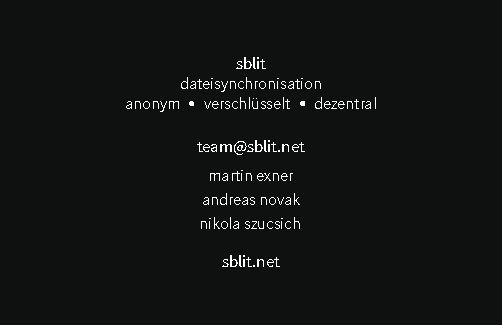
\includegraphics[width=85mm,height=55mm]{images/visitenkarte_rueckseite.pdf}
    \caption{Visitenkarte}
\end{figure}

\voffset10mm

\printindex{}

\bibliographystyle{plaindin}
\bibliography{diplom}

\printglossary[type=\acronymtype]
\printglossary

\end{document}
